\documentclass{article}
\usepackage{hyperref}
\usepackage{graphicx}
\usepackage[a4paper, left = 3.5cm, right = 3.5cm, top = 3.5cm, bottom = 3.5cm ]{geometry}
\usepackage{minted}
\usepackage{subfig}
\usepackage{bm}
\hypersetup{
	colorlinks,
	citecolor=black,
	filecolor=black,
	linkcolor=black,
	urlcolor=black
}
\begin{document}

	
	\begin{titlepage}
		
		\title{Progetto di Introduzione Intelligenza Artificiale\\Blocks World}
		\author{Studente: Diego Arcelli\\Docente: Prof. Valentina Poggioni\\Assistenti alla didattica: Dr. Alina Elena Baia, Dr. Gabriele Di Bari}
		\date{A.A. 2020/2021}
		\maketitle
		\centering
		
\includegraphics[width=10cm]{./images/logo_unipg.png}\hspace{-1cm}
		
	\end{titlepage}
	
	\tableofcontents
	\newpage
	
	\section{Descrizione del problema}
	\subsection{Descrizione ad alto livello}
	Blocks World è un dominio dell'intelligenza artificiale in cui si ha un insieme di blocchi numerati disposti su una superficie piana e un braccio meccanico che può spostare i blocchi. Si vuole realizzare un programma che implementi Blocks World, acquisendo come input due immagini, una raffigurante la configurazione iniziale dei blocchi e l'altra raffigurante la configurazione finale, e restituisca come output la sequenza di azioni che il braccio deve effettuare per passare dalla configurazione iniziale alla configurazione finale.
	
	\subsection{Definizione formale e vincoli}
	Il problema è stato modellato tenendo conto dei seguenti vincoli:
	\begin{enumerate}
		\item L'ambiente è un mondo 2-dimensionale di altezza e larghezza finita.
		\item I blocchi sono quadrati tutti della stessa dimensione.
		\item I blocchi devono essere numerati in maniera sequenziale (partendo da 1).
		\item Il massimo numero di blocchi presenti in un istanza del mondo è 6.
		\item Vi è un numero fisso di aree nella mappa, ordinate da sinistra verso destra, dove si possono formare colonne di blocchi.
		\item Un blocco può appartenere ad una sola area (non può essere a cavallo di più aree).
		\item L'altezza della mappa è espressa come numero intero che indica il massimo numero di blocchi che è possibile impilare uno sopra l'altro.
		\item La larghezza della mappa è espressa come un numero intero che indica il numero di aree del mondo dove si possono formare colonne di blocchi.
		\item In ogni possibile configurazione del mondo l'altezza è data dal numero di blocchi presenti nella specifica istanza del mondo (quindi può valere al più 6).
		\item La larghezza della mappa può essere stabilita in maniera arbitraria.
		\item Il braccio meccanico può spostare solo un blocco alla volta.
		\item Il braccio meccanico può prelevare per lo spostamento solo i blocchi che non hanno sopra di loro altri blocchi.
		\item Quando un blocco viene scelto per essere spostato dal braccio meccanico non può essere rimesso dove è stato prelevato.
		\item I blocchi possono essere posizionati solo sopra altri blocchi o sulla superficie del mondo (ovvero i blocchi non possono fluttuare).
		\item Per valutare la qualità del lavoro svolto dal braccio per portare il mondo dallo stato iniziale allo stato finale si usa come metrica il numero di blocchi spostati.
	\end{enumerate}
	Un altro modo per visualizzare il mondo è quello di pensarlo come una matrice di dimensione $h \times w$ (dove $h$ è l'altezza del mondo e $w$ è la larghezza) in cui ogni blocco ha una posizione indicata da una coppia di indici (uno per la riga uno per la colonna) che devono ovviamente rispettare i vincoli sopra elencati. Questa rappresentazione è quella che verrà anche utilizzata per l'implementazione del problema.\\
	Di seguito verranno mostrati alcuni esempi di raffigurazioni di istanze di possibili mondi. La figura \ref{fig:valid} mostra un esempio di configurazione valida di 6 blocchi, in un mondo di altezza 6 e larghezza 7 (notare che anche se dall'immagine sembra inferiore, l'altezza del mondo è comunque 6 per il vincolo numero 9). La figura \ref{fig:matrix} mostra due configurazioni di altezza 6 e larghezza 5, evidenziando la struttura a matrice del mondo. Ad esempio nella figura a sinistra la posizione del blocco 1 è rappresentata dalla coppia di indici riga-colonna (0,1) e la posizione del blocco 2 dalla coppia (2,1). Da notare come la configurazione a destra non è valida in quanto il blocco 2 è cavallo tra le posizioni (2,1) e (2,2), violando dunque il vincolo numero 6.
	\begin{figure}[H]
	\centering
	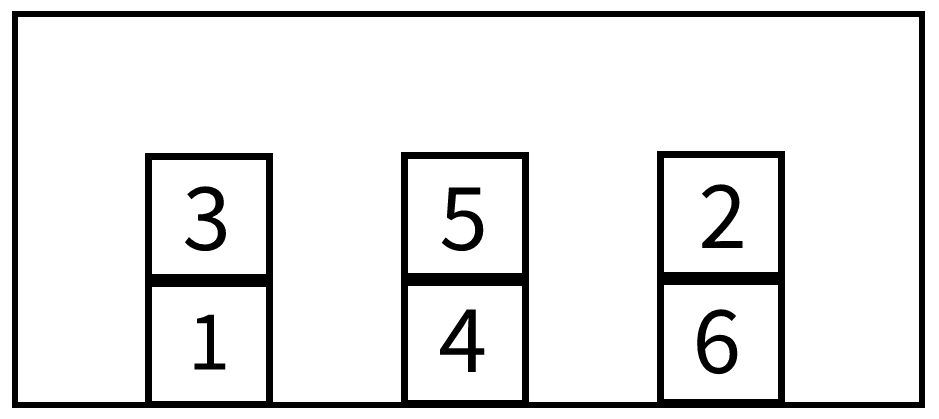
\includegraphics[width=10cm]{./images/valid.png}
	\caption{Esempio di una configurazione con 6 blocchi valida}
	\label{fig:valid}
	\end{figure}
	\begin{figure}[H]
	\centering
	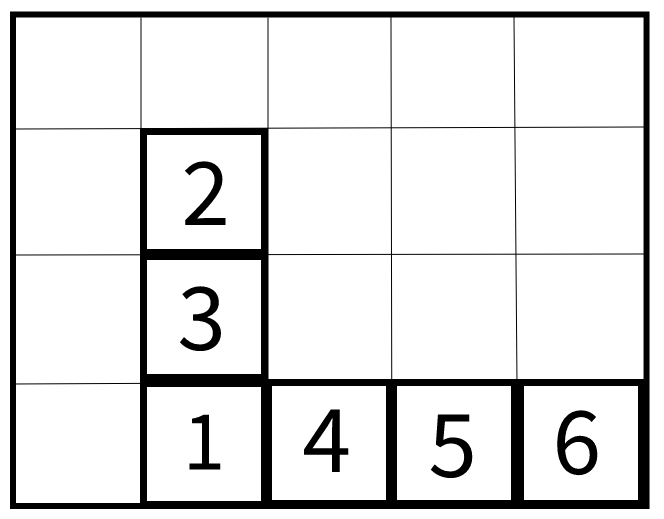
\includegraphics[width=6cm]{./images/valid-grid.png}
	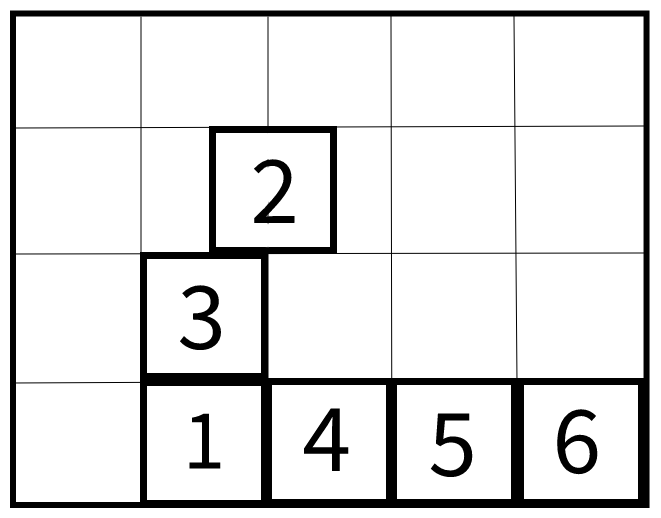
\includegraphics[width=6cm]{./images/non-valid-grid.png}
	\caption{Configurazioni che evidenziano la struttura a matrice del mondo}
	\label{fig:matrix}
	\end{figure}

	\noindent Le immagini nella figura \ref{fig:non-valid} invece sono una rappresentazione di due configurazioni non valide. In particolare quella di sinistra viola il vincolo numero 3 (la numerazione di blocchi non è sequenziale), mentre l'immagine di destra viola il vincolo numero 14 (il blocco numero 4 sta fluttuando).

	\begin{figure}[H]
	\centering
	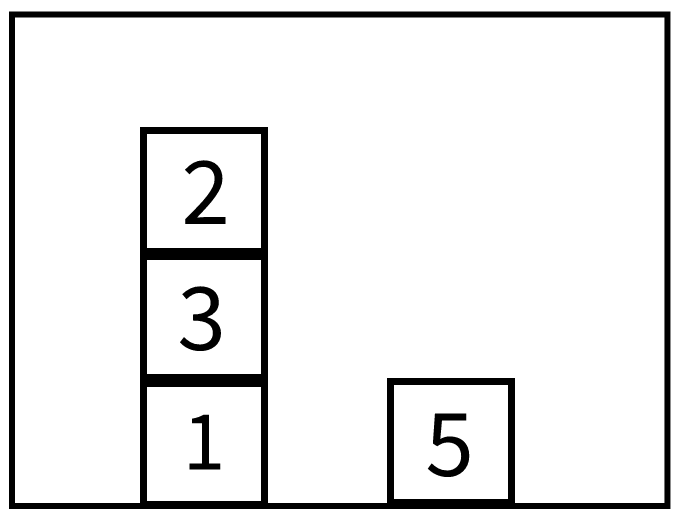
\includegraphics[width=6cm]{./images/non-valid-1.png}
	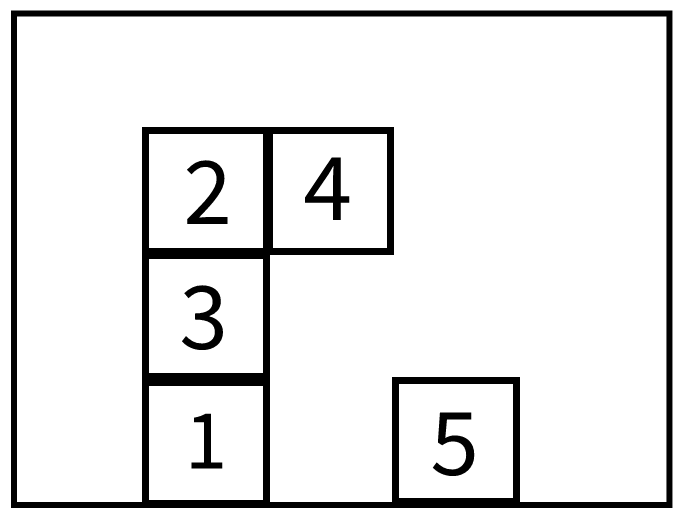
\includegraphics[width=6cm]{./images/non-valid-2.png}
	\caption{Esempi di due configurazioni non valide}
	\label{fig:non-valid}
	\end{figure}
	
	\subsection{Struttura del programma}
	Il programma realizzato per presentare un'implementazione di Blocks World è strutturato in tre moduli:
	\begin{itemize}
		\item Il primo fa uso del modulo AIMA di Python per modellare il problema, fornendo una rappresentazione degli stati che poi può essere utilizzata dagli algoritmi di ricerca per fornire una soluzione. I file che fanno riferimento a questo modulo sono: \verb*|blocks_world.py| e \verb*|search_algs.py|.
		\item Il secondo fa uso della libreria per la manipolazione di immagini OpenCV, per estrarre dalle immagini, raffiguranti la configurazione iniziale e la configurazione finale, la corretta rappresentazione degli stati da passare al modulo di AIMA. Il file che fa riferimento a questo modulo è \verb*|load_state.py|.
		\item Il terzo si occupa dell'addestramento di una rete neurale convoluzionale, per il riconoscimento di cifre scritte a mano, facendo uso del dataset del MNIST. Tale modulo servirà a quello di OpenCV per interpretare le cifre scritte sui blocchi. Il file che fa riferimento a questo modulo è \verb*|cnn.py|.
	\end{itemize}
	L'interazione tra l'utente ed il programma può avvenire mediante un'interfaccia grafica realizzata con il modulo di Python Tkinter (file \verb*|launch.py|) o tramite uno script che può essere eseguito da linea di comando (file \verb*|main.py|).

	\section{Definizione del probelma con AIMA}
	\subsection{Rappresentazione degli stati}
	Gli stati vengono rappresentati nella seguente maniera:
	\begin{itemize}
		\item Una lista di triple di numeri interi (una per ogni blocco) che rappresentano:
		\begin{enumerate}
			\item Il numero che identifica il blocco.
			\item La posizione del blocco nell'asse verticale.
			\item La posizione del blocco nell'asse orizzontale.
		\end{enumerate}
		\item La larghezza della specifica istanza del mondo.
	\end{itemize}
	Prendiamo come esempio la seguente rappresentazione:
	\begin{minted}{python}
((1,0,0), (2,1,0), (3,0,2), (4,0,4), 6)
	\end{minted}
	essa rappresenta lo stato raffigurato nella figura \ref{fig:state_ex}.
	\begin{figure}[H]
		\centering
		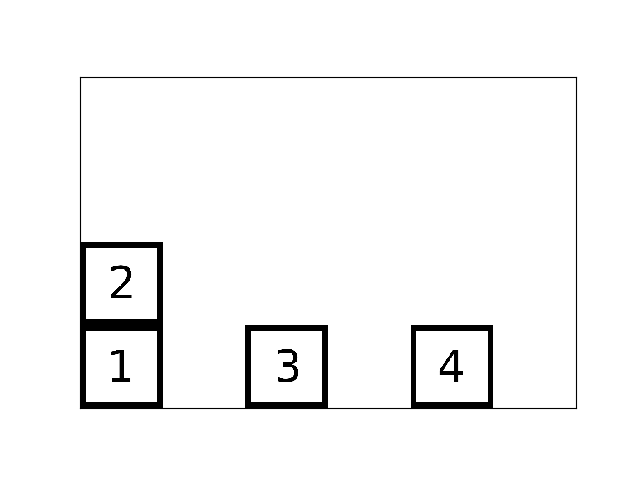
\includegraphics[width=8cm]{./images/example_state.png}
		\caption{Rappresentazione di uno stato}
		\label{fig:state_ex}
	\end{figure}
	
	\subsection{Rappresentazione delle azioni}
	Le azioni effettuabili in un particolare stato sono rappresentate come una lista di triple (una per ogni possibile azione) di numeri interi. Gli elementi delle triple rappresentano:
	\begin{enumerate}
		\item Il numero del blocco da spostare.
		\item La nuova posizione sull'asse verticale del blocco.
		\item La nuova posizione sull'asse orizzontale del blocco.
	\end{enumerate}
	Prendiamo ad esempio il seguente stato:
	\begin{minted}{python}
((1,0,0), (2,1,0), (3,0,2), 3)
	\end{minted}
	la sua rappresentazione grafica può essere visualizzata nella figura \ref{fig:actions}.
	\begin{figure}[H]
		\centering
		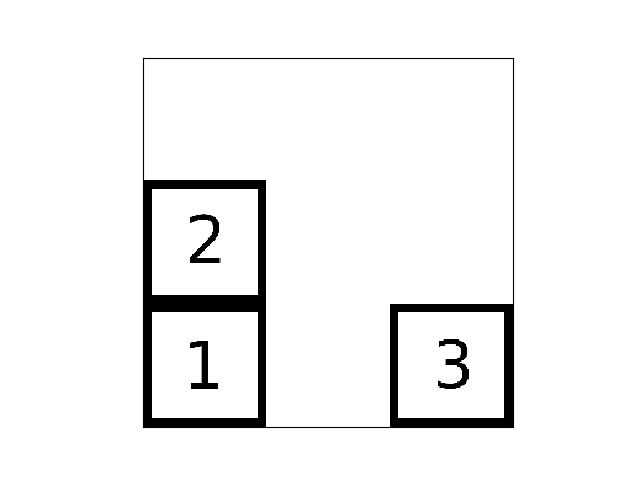
\includegraphics[width=8cm]{./images/action_example.png}
		\caption{Stato di esempio per la rappresentazione delle azioni}
		\label{fig:actions}
	\end{figure}
	\noindent Le azioni effettuabili nello stato vengono rappresentate nella seguente maniera:
	\begin{minted}{python}
[(2,0,1), (2,1,2), (3,2,0), (3,0,1)]
	\end{minted}
	ad esempio la prima tripla rappresenta lo spostamento del blocco 2 tra il blocco 1 e 3, mentre la seconda rappresenta lo spostamento lo spostamento del blocco 2 sopra il blocco 3.
	\section{Elaborazione immagini ed estrazione degli stati}
	\subsection{Formato delle immagini}
	Come già spiegato, il programma prevede l'acquisizione di due immagini raffiguranti lo stato iniziale e lo stato finale del mondo. Le immagini da acquisire dovranno rispettare alcuni vincoli:
	\begin{itemize}
		\item I blocchi devono essere disegnati in un box rettangolare che serve all'algoritmo sia per facilitare la rilevazione dei blocchi, che per stabilire la larghezza del mondo.
		\item I blocchi del livello più basso (quelli con altezza 0) devono essere appoggiati alla parte inferiore del box.
		\item Ogni blocco deve avere disegnata al suo interno la cifra che lo identifica.
		\item Tutte le linee disegnate devono essere continue.
	\end{itemize}
	
	\subsection{Illustrazione del processo}

	Per comprendere come funziona l'elaborazione delle immagini verrà illustrato il procedimento nella seguente immagine:\\
	
	\begin{figure}[H]
		\centering
		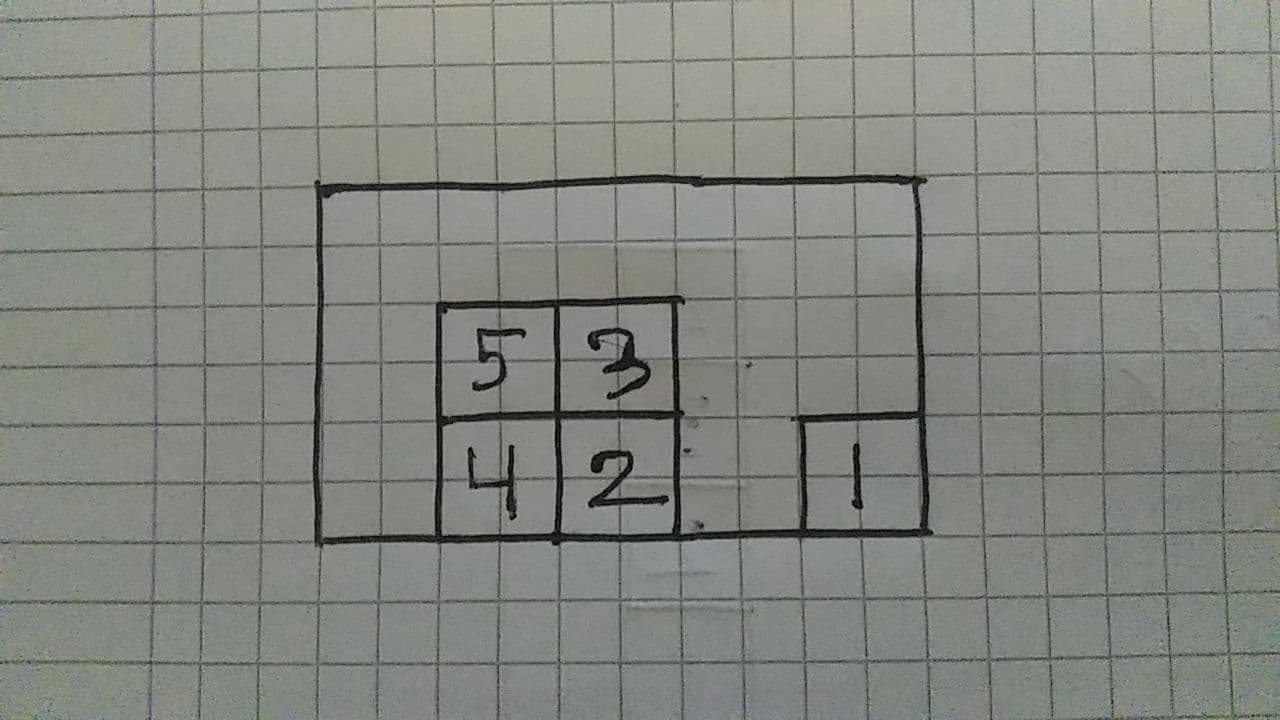
\includegraphics[width=8cm]{./images/immagine_test.jpg}
	\end{figure}


	\noindent Per prima cosa l'immagine vien convertita da RGB a scala di grigi, per lavorare con un solo canale:
	
	\begin{figure}[H]
		\centering
		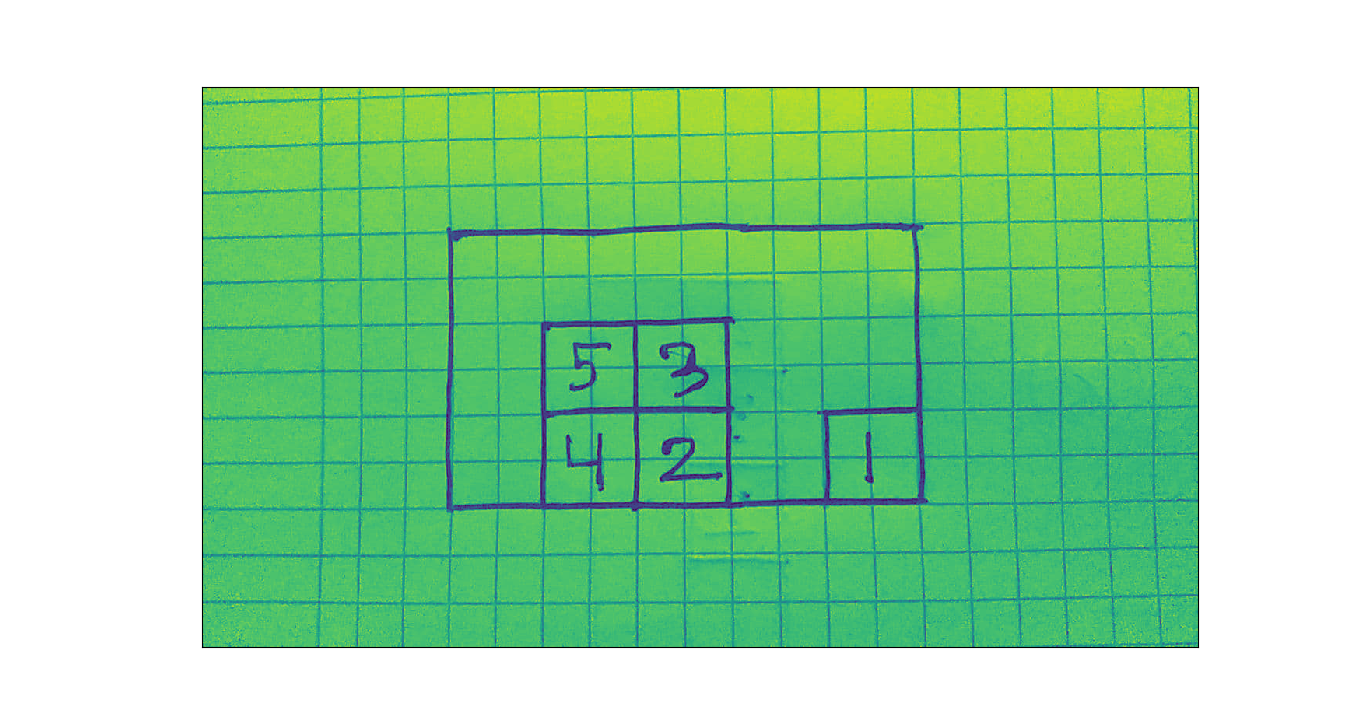
\includegraphics[width=11cm]{./images/immagine_test_gray.png}
	\end{figure}
	
	
	\noindent L'immagine in scala di grigi viene sottoposta a varie trasformazioni, allo scopo di evidenziare le linee relative al box dei blocchi ed eliminare tutto il resto. In particolare:
	\begin{enumerate}
		\item Viene aggiunto un effetto di blur all'immagine (gaussian blur e median blur)
		\item Si applica median thresholding per mettere in evidenza le linee disegnate
		\item Si riapplica l'effetto blur e si erodono un po' le linee nere per eliminare eventuali punti neri o linee sottili rimaste nell'immagine.
		\item Si individua il contorno degli elementi rimanenti nell'immagine e si rimuovono quelli la cui area e inferiore ad una determinata soglia rispetto all'area dell'immagine intera
	\end{enumerate}
	L'effetto prodotto è il seguente:
	
	\begin{figure}[H]
		\centering
		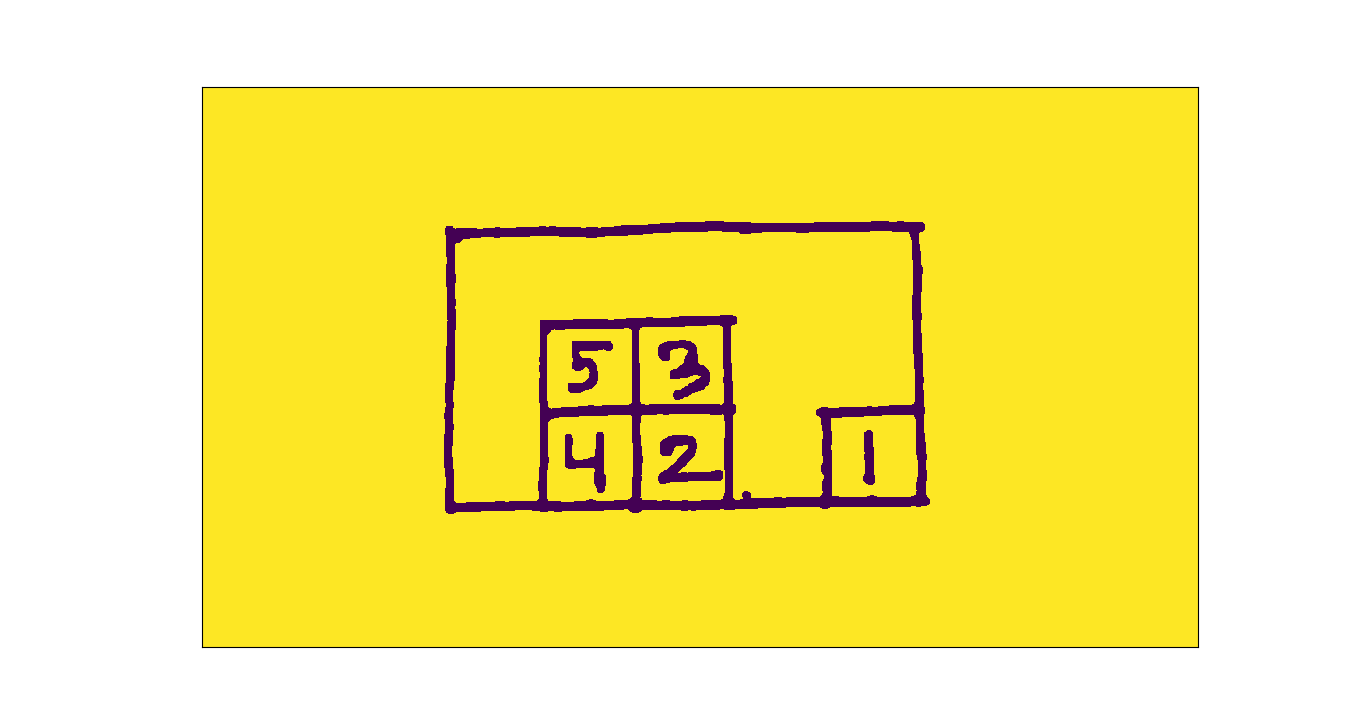
\includegraphics[width=11cm]{./images/immagine_test_filtered.png}
	\end{figure}
	
	\noindent Tramite la funzione findContours di OpenCV si individuano i contorni dell'immagine, e si prende quello con l'area maggiore, che dovrà essere quello che contiene il box dei blocchi, in maniera tale da poter lavorare direttamente su quella porzione di immagine:
	
	\begin{figure}[H]
		\centering
		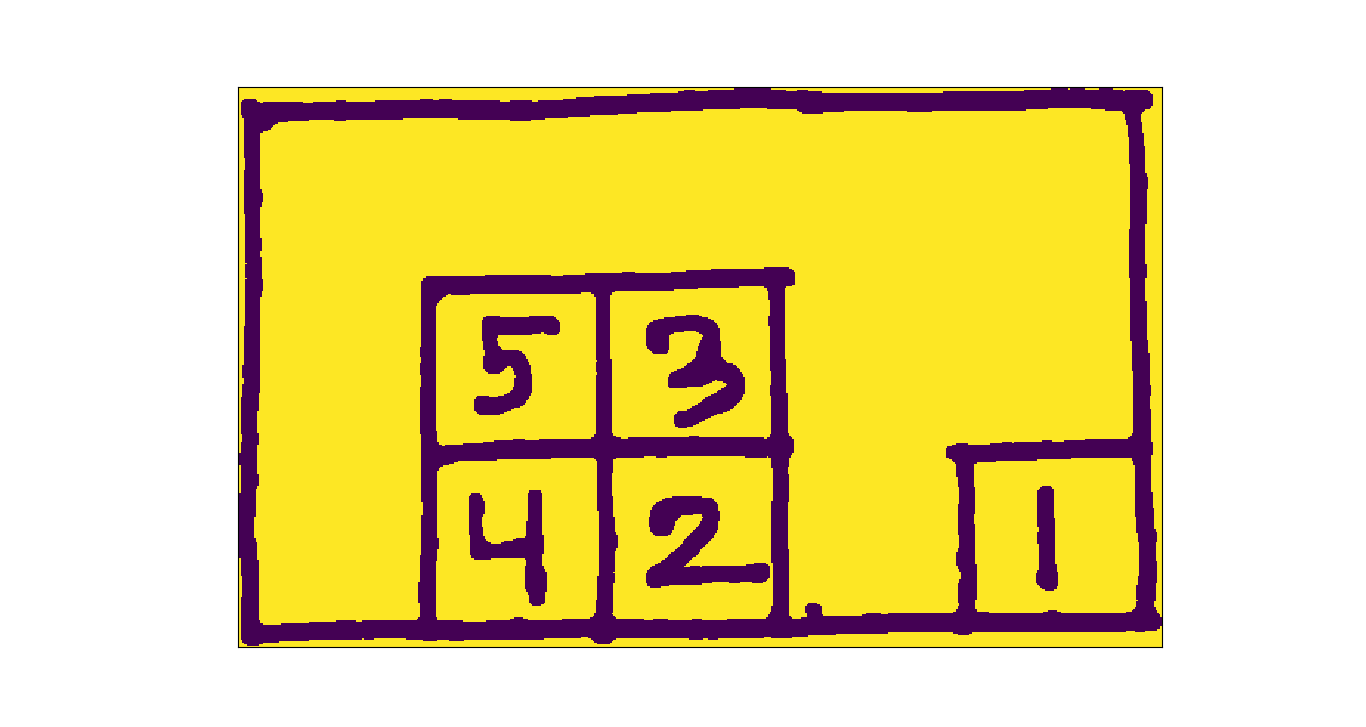
\includegraphics[width=11cm]{./images/immagine_test_box.png}
	\end{figure}
	
	\noindent Successivamente si individuano i contorni dell'immagine tramite la funzione \verb*|findContours| di OpenCV, che permette anche di individuare la loro relazione gerarchica e quindi capire quali sono i contorni più interni (contorni contenuti in altri contorni). Tramite questo meccanismo si possono individuare i numeri che identificano i blocchi:
	
	\begin{figure}[H]
		\centering
		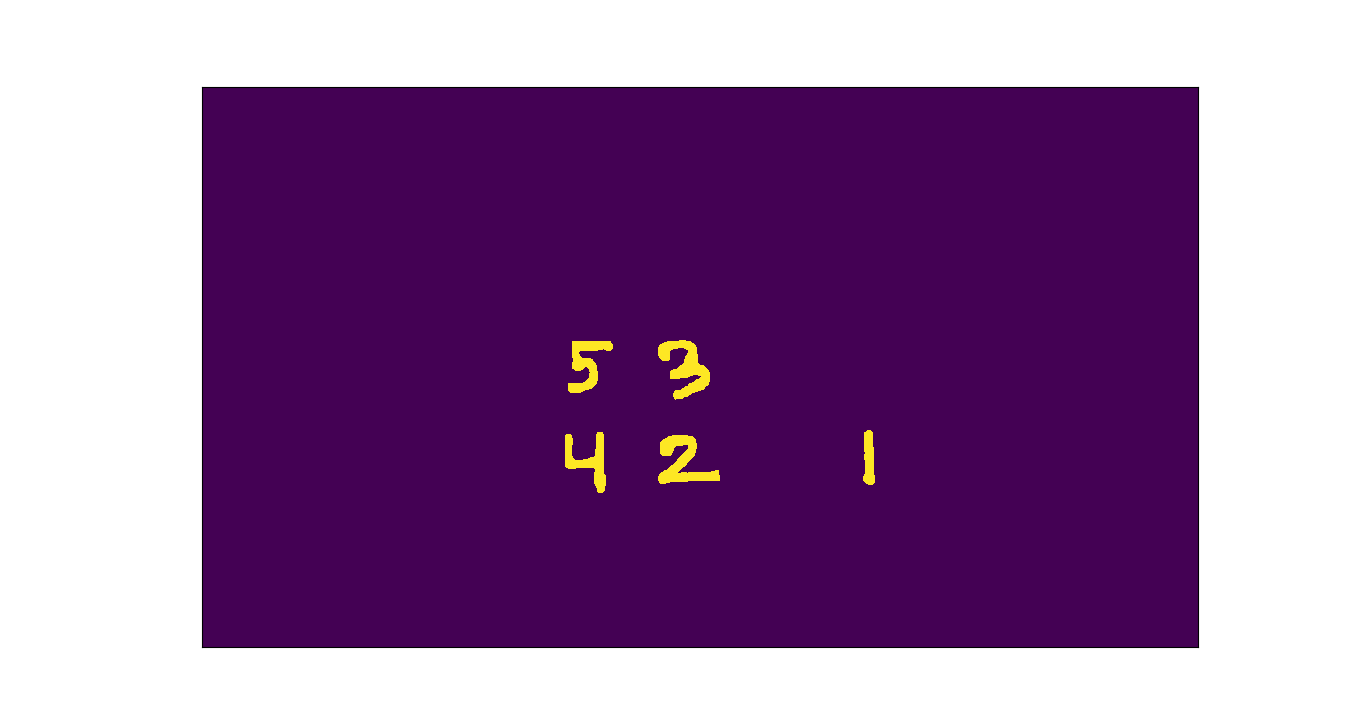
\includegraphics[width=11cm]{./images/immagine_test_numeri.png}
	\end{figure}
	
	
	\noindent A questo punto si possono analizzare le cifre una per una, passandole alla rete neurale per il riconoscimento e memorizzandone la posizione all'interno del box:
	
	\begin{figure}[H]
		\centering
		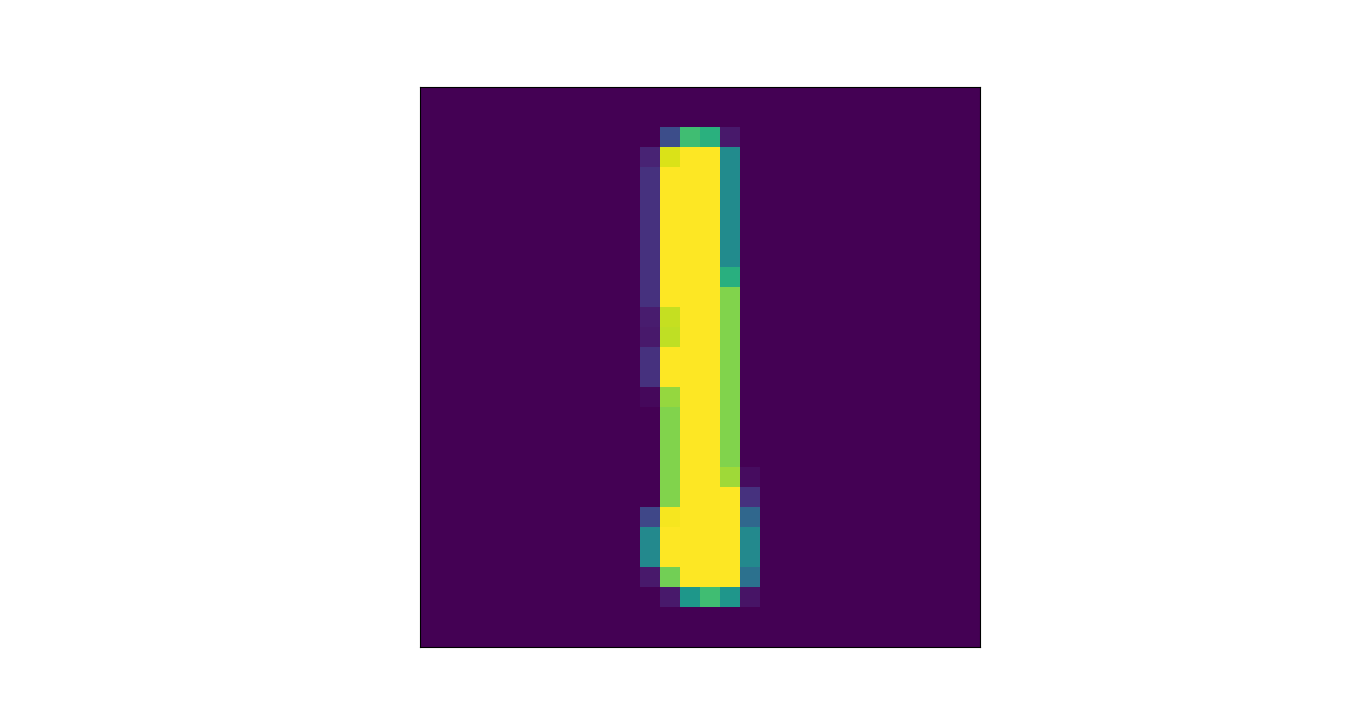
\includegraphics[width=2.5cm]{./images/1.png}
		
\includegraphics[width=2.5cm]{./images/2.png}
		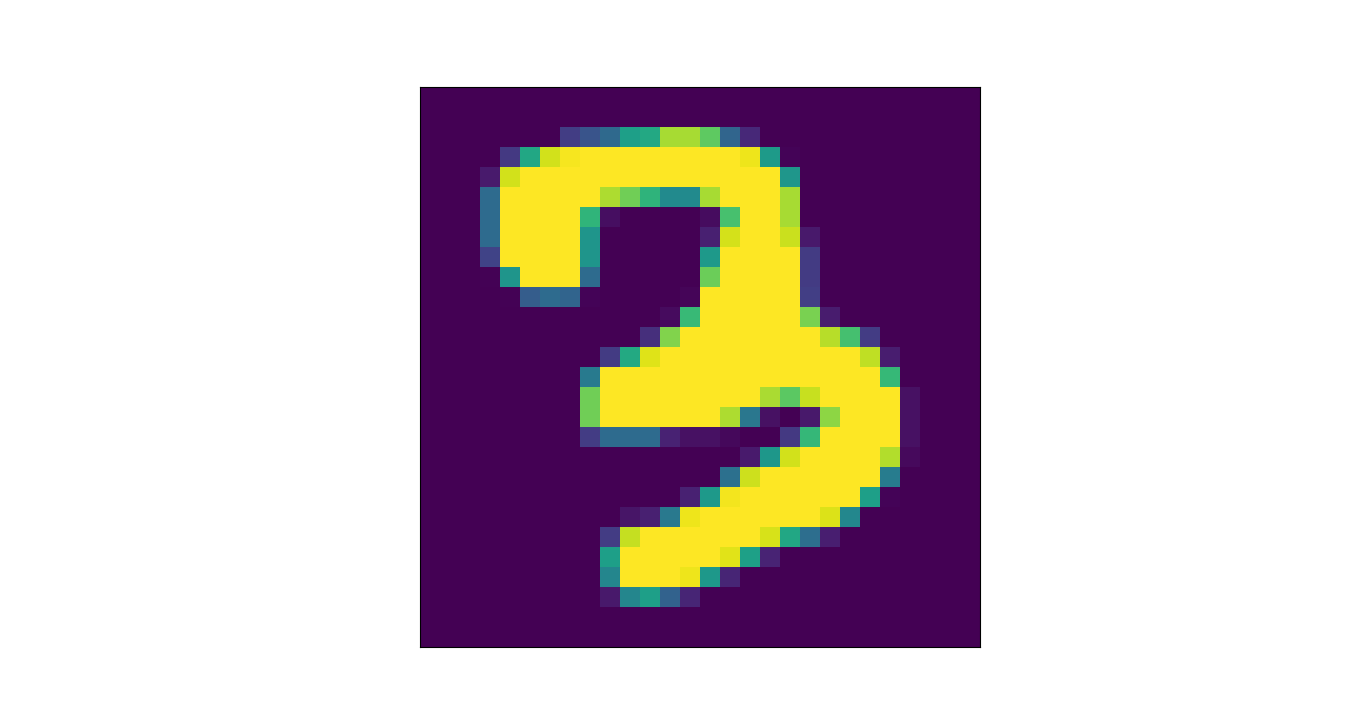
\includegraphics[width=2.5cm]{./images/3.png}
		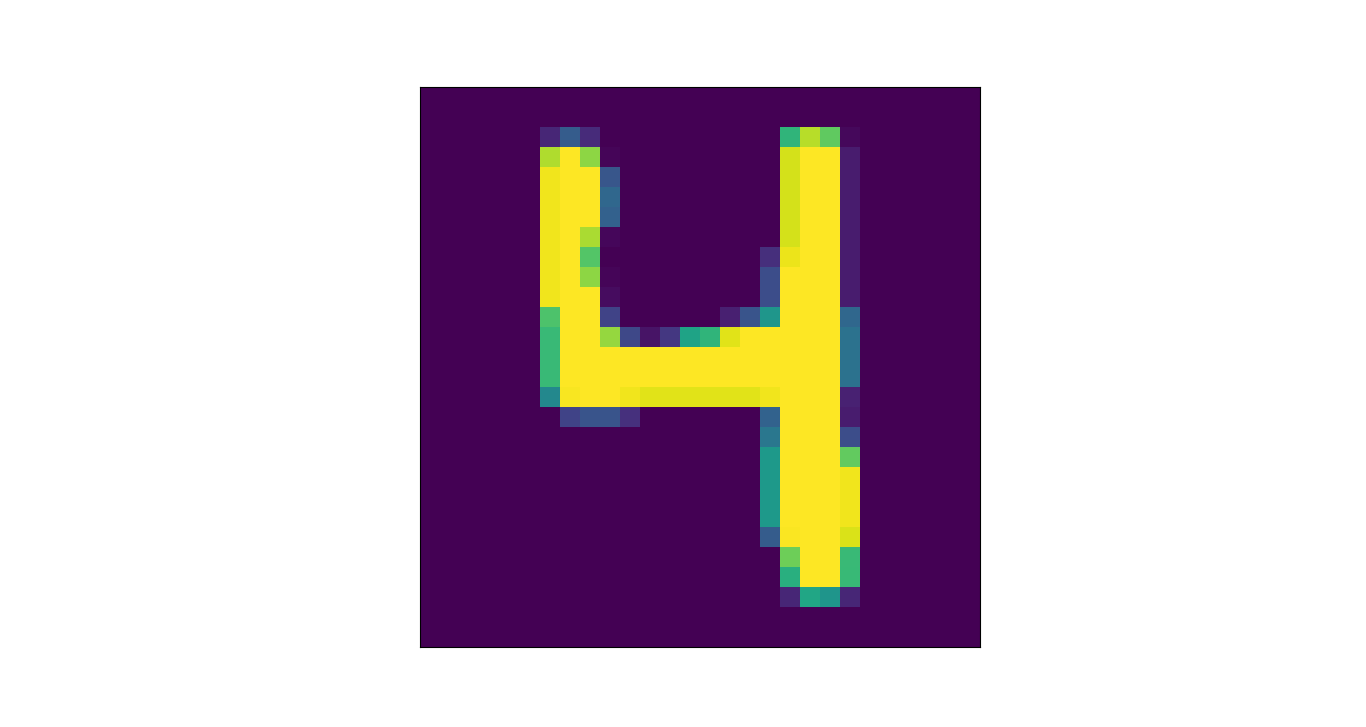
\includegraphics[width=2.5cm]{./images/4.png}
		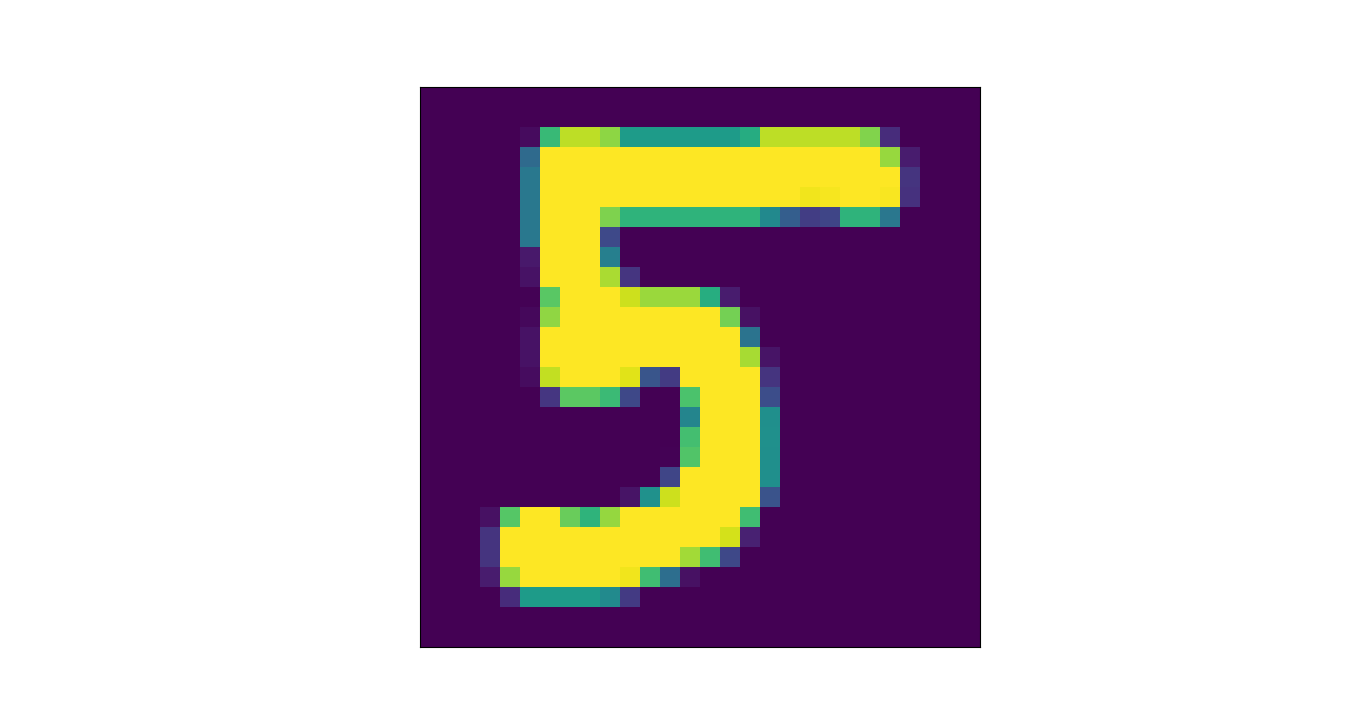
\includegraphics[width=2.5cm]{./images/5.png}
	\end{figure}

	
	\noindent Una volta ottenuto la posizione delle cifre è facile individuare i blocchi che le contengono. Partendo dalla posizione dei blocchi si può calcolare la distanza tra di loro e dai bordi del box, in maniera tale da ottenere la larghezza dello stato, le dimensioni dei blocchi e la posizione dei blocchi all'interno del box:
	
	
	\begin{figure}[H]
		\centering
		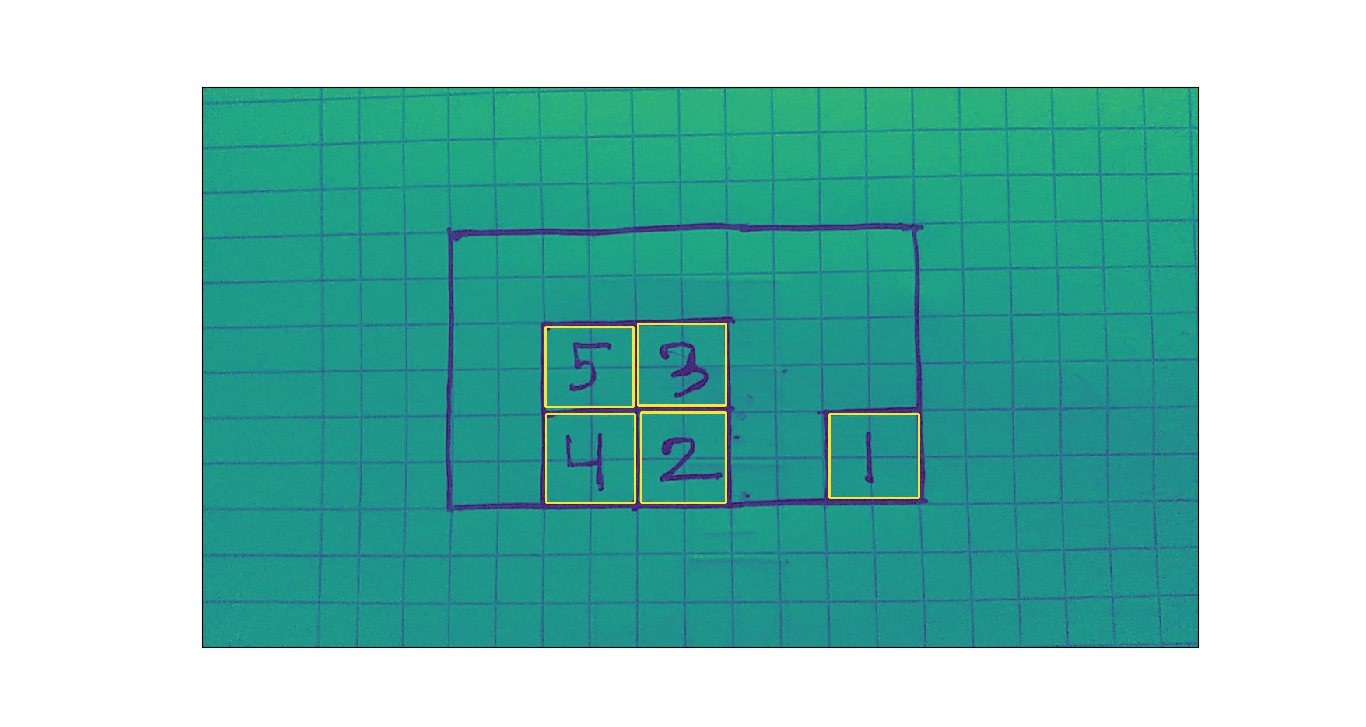
\includegraphics[width=11cm]{./images/immagine_test_digits.png}
	\end{figure}

	\noindent Da queste informazioni si può costruire lo stato (come è stato definito in precedenza) per passarlo al modulo di AIMA:
	
	\begin{minted}{python}
((4,0, 1), (5,1,1), (2,0,2), (3,1,2), (1,0,4), 5)
	\end{minted}
	
	\subsection{Suggerimenti}
	Il processo è un po' artificioso ma, dai test che sono stati effettuati, permette di estrarre correttamente lo stato dall'immagine in moltissimi casi. Per migliorare la precisione è bene seguire i seguenti accorgimenti:
	\begin{itemize}
		\item Assicurarsi che l'illuminazione dell'immagine sia distribuita in maniera uniforme (aree più illuminate di altre potrebbero compromettere il processo).
		\item Assicurarsi che le linee disegnate non presentino discontinuità.
		\item Se si usa un foglio a quadretti per disegnare lo stato, assicurarsi che il tratto della penna utilizzata sia abbastanza più marcato delle linee del foglio.
		\item Assicurarsi che l'angolazione dalla quale viene scattata la foto sia perpendicolare al foglio, in maniera tale che le aree dei rettangoli che definiscono il box e i blocchi non risultino alterate.
		\item Assicurarsi che non vi siano altri elementi di disturbo non necessari presenti nell'immagine.
	\end{itemize}



	\section{Riconoscimento delle cifre}
	Per il riconoscimento le cifre che identificano i blocchi è stata utilizzata una rete neurale convoluzionale addestrata sul dataset del MNIST. Entrando maggiormente nel dettaglio la struttura della rete è la seguente:
	\begin{enumerate}
		\item Input un immagine 28$\times$28 con un solo canale
		\item Un layer convoluzionale che produce 24 filtri, con kernel 3$\times$3 e ReLU come funzione di attivazione
		\item Un layer di pooling con kernel 2$\times$2
		\item Un layer di dropout con rate 0.5
		\item Un secondo layer convoluzionale che produce 36 filtri con kernel 3$\times$3 e ReLU come funzione di attivazione
		\item Un secondo layer di max pooling con kernel 2$\times$2
		\item Un secondo layer di dropout con layer 0.5
	\end{enumerate}
	Dopodiché inizia la parte della rete di tipo MLP:
	\begin{enumerate}
		\setcounter{enumi}{5}
		\item Il layer di input composto da 900 neuroni
		\item Un primo hidden layer di 128 neuroni e ReLU come funzione di attivazione
		\item Il layer di output di 10 neuroni (uno per ogni cifra) e softmax come funzione di attivazione
	\end{enumerate}
	Si è allenato il modello utilizzando un batch di 64 immagini. Dopo alcuni test si è valutato che il numero ottimale di epoche per addestrare il modello era di 10, in quanto con numeri maggiori l'accuracy nel validation set o incrementava di pochissimo o addirittura si riduceva (probabilmente il modello andava in overfitting). Si è utilizzato Adam come ottimizzatore, la sparse categorical crossentropy come funzione per misurare l'errore e l'accuracy come metrica per misurare la precisione. L'andamento dell'accuracy e dell'errore nel training set e nel validation set sono riportati nelle figure \ref{fig:accuracy} e \ref{fig:loss}.
	\begin{figure}[H]
		\centering
		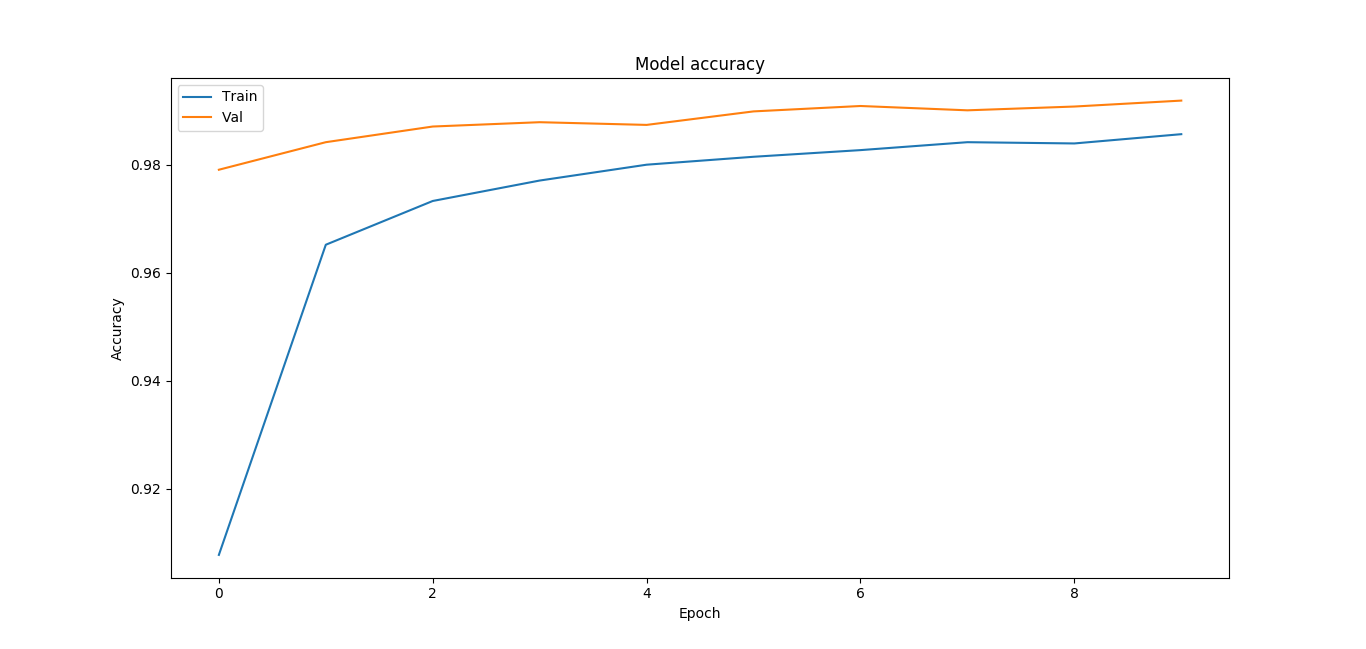
\includegraphics[width=10cm]{./images/accuracy.png}
		\caption{Andamento dall'accuracy durante l'addestramento}
		\label{fig:accuracy}
	\end{figure}
	\begin{figure}[H]
		\centering
		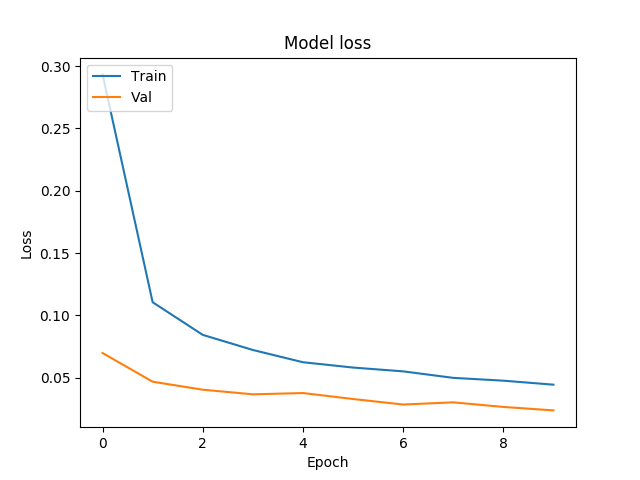
\includegraphics[width=10cm]{./images/loss.png}
		\caption{Andamento dall'errore nel durante l'addestramento}
		\label{fig:loss}
	\end{figure}



	\let\footnoterule\relax
	\section{Statistiche deggli algoritmi di ricerca}
	\subsection{Algoritmi di ricerca}
	Gli algoritmi implementati sono i seguenti:
	\begin{itemize}
		\item Depth First Search (DFS)
		\item Breadth First Search (BFS)
		\item Iterative Deepening Search (IDS)
		\item Uniform Cost Search (UCS)
		\item Recursive Best First Search (RBFS)
		\item A*
	\end{itemize}
	Di seguito sono riportate alcune informazioni sull'implementazione degli algoritmi importanti per poter interpretare i risultati degli esperimenti.\\Sebbene IDS e DFS applichino lo stesso tipo di ricerca (in profondità) nell'implementazione della DFS, quando si espande un nodo, prima prima si generano tutti i figli e poi si procede con l'espansione di uno di essi, mentre nell'implmentazione della IDS appena si genera un figlio si procede alla sua espansione. Quindi nel caso della IDS la complessità in spazio sarà $O(d)$\footnote{$d$ è la profondità più bassa per una soluzione, $b$ è il branching factor, $m$ è la massima profondità}, mentre nel caso della DFS sarà $O(bm)$.\\
	Per quanto riguarda l'UCS la funzione di costo (in rispetto al vincolo numero 15) è quella di costo unitario, ovvero ogni azione ha costo 1. Questo fa si che la ricerca avvenga per livelli come nel caso della BFS, l'unica differenza è che nella BFS il goal test viene effettuato quando il nodo viene aggiunto alla frontiera, mentre nel caso della UCS viene effettuato in fase di espansione del nodo.\\
	Nel caso di A* e RBFS la funzione euristica $h$ utilizzata è semplicemente il numero di blocchi nella posizione errata (ovviamente rispetto allo stato finale). Prendiamo ad esempio la figura \ref{fig:euristica}.
	\begin{figure}[H]
		\centering
		\subfloat[Stato iniziale]{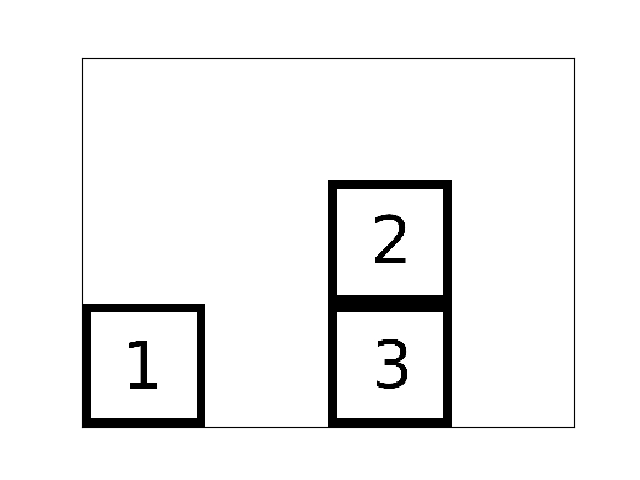
\includegraphics[scale=0.4]{./images/heuristic_ex_1.png}
		}
		\subfloat[Stato finale]{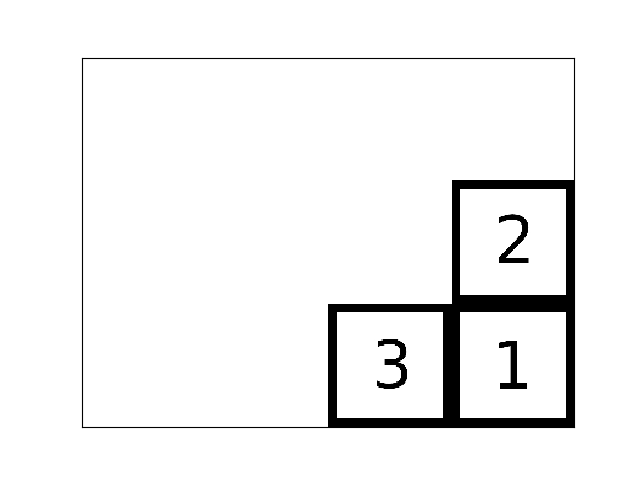
\includegraphics[scale=0.4]{./images/heuristic_ex_2.png}
		}    
		\protect\caption{Esempio per la funzione euristica}
		\label{fig:euristica}
	\end{figure}

	\noindent Il valore della funzione euristica nello stato nell'immagine \ref{fig:euristica}a vale 2, in quanto il blocco 3 è nella posizione corretta mentre il blocchi 1 e 2 no. Tale funzione euristica è:
	\begin{itemize}
		\item Ammissibile: in quanto per portare il mondo dalla sua configurazione attuale a quella corretta, i blocchi nella posizione errata andranno spostati almeno una volta.
		\item Consistente: se il valore della funzione euristica in un determinato stato $s$ è $h(s)$, spostando un blocco e passando allo stato $s'$ con l'azione $a$ il valore della funzione di costo $g(s,a,s')$, per come è stato definito il problema, sarà sempre pari ad 1 per ogni possibile $a$. Si ricorda che $h$ è consistente se vale la seguente disuguaglianza: 
		$h(s) \leq h(s') + g(s,a, s')$ per ogni possibile coppia $(s,s')$, che nel nostro caso diventa $h(s) \leq h(s') + 1$. Per quanto riguarda $h(s')$ si hanno tre casi: 
		\begin{enumerate}
			\item Un blocco in una posizione errata è stato spostato in un altra posizione errata, dunque $h(s') = h(s)$. In tal caso si avrà che $h(s) \leq h(s) + 1$.
			\item Un blocco in una posizione corretta viene spostato in una posizione errata, quindi si avrà che $h(s') = h(s) + 1$. In tal caso si avrà che $h(s) \leq h(s) + 1 + 1 = h(s) + 2$.
			\item Un blocco in una posizione errata viene spostato nella posizione corretta, quindi $h(s') = h(s) - 1$. In tal caso si avrà che $h(s) \leq h(s) - 1 + 1 = h(s)$
		\end{enumerate}
	\end{itemize}
	Tale funzione euristica corrisponde ad un rilassamento del problema nel quale due blocchi possono essere invertiti di posizione con una sola azione.
	
	\subsection{Esperimenti}
	\subsubsection{Configurazione degli esperimenti}
	I test condotti per misurare la qualità delle ricerche tengono in considerazione i seguenti fattori:
	\begin{itemize}
		\item Il numero di nodi espansi durante la ricerca ($n$).
		\item Il massimo numero di nodi presente nella frontiera in un qualsiasi momento della ricerca ($m$).
		\item Il numero medio di nodi presente nella frontiera  durante la ricerca ($\mu$).
		\item La lunghezza della soluzione ($l$).
	\end{itemize}
	Il numero medio di nodi $\mu$ è stato calcolato utilizzando la seguente formula:\\
	\[ \mu = \Bigl\lfloor \frac{1}{n}\sum_{i=1}^{n} n_{i} \Bigl\rfloor\]
	Dove $n$ è il numero di nodi espansi durante la ricerca e $n_{i}$ è il numero di nodi presenti nella frontiera all'$i$-esima espansione. 
	
	\subsubsection{Primo test}
	Il primo test è stato condotto in un mondo molto semplice con soli tre blocchi, rappresentato dalle immagini nella seguente figura \ref{fig:exp1}.
	\begin{figure}[H]
		\centering
		\subfloat[Stato iniziale]{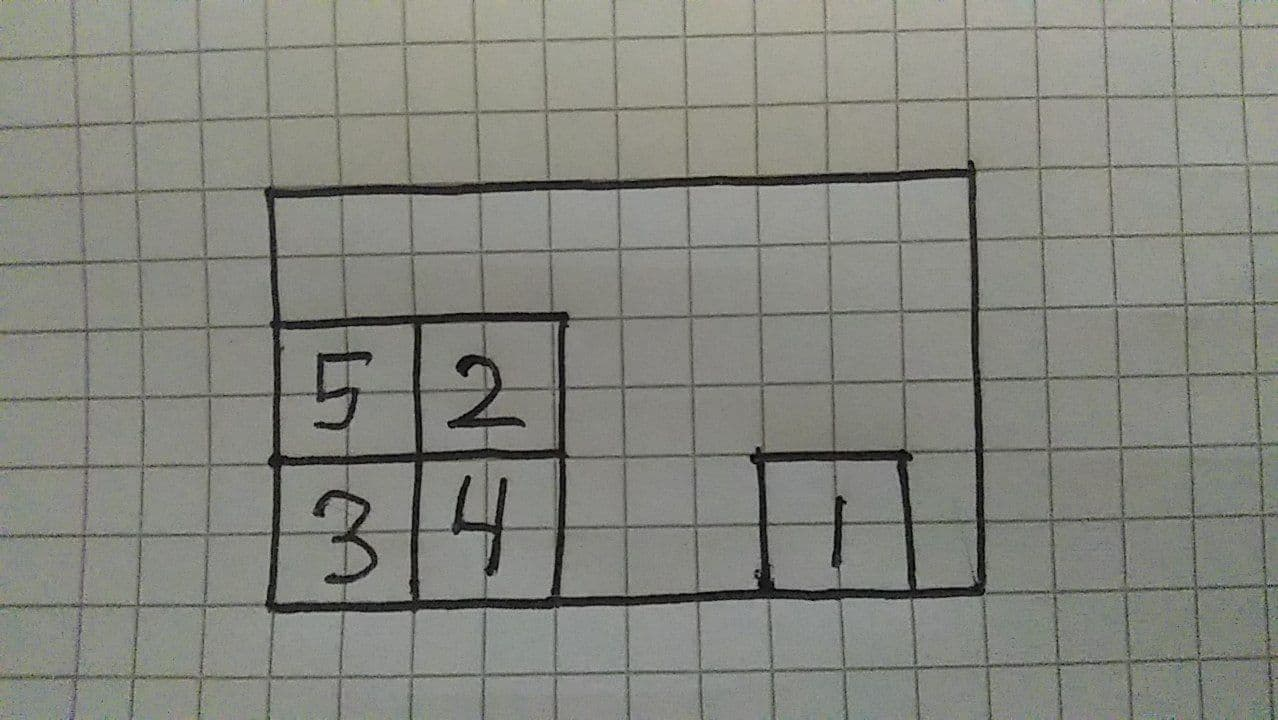
\includegraphics[width=6cm]{../images/sample0/initial.jpg}
		}
		%  No blank line
		\subfloat[Stato finale]{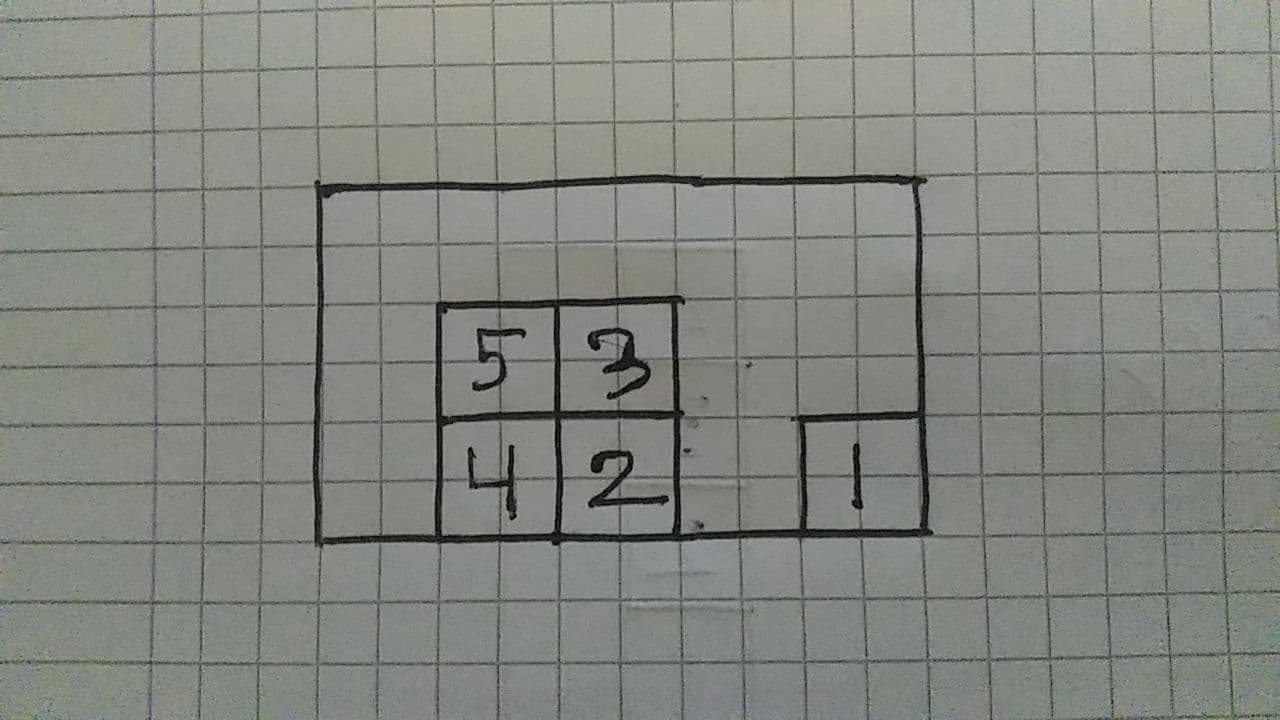
\includegraphics[width=6cm]{../images/sample0/goal.jpg}
		}    
		\protect\caption{Configurazioni per il primo test}
		\label{fig:exp1}
	\end{figure}
	
	\noindent Le due immagini vengono elaborate e codificate correttamente nei seguenti stati:
	\begin{minted}{python}
		initial = ((1,0,0), (3,1,0), (2,0,1), 3)
		goal    = ((3,0,1), (1,0,2), (2,1,2), 3)
	\end{minted}
	Le performance dei vari algoritmi di ricerca sono riassunte nella tabella \ref{tab:exp1}.
	\begin{table}[H]
		\centering
		\def\arraystretch{1.5}
		\begin{tabular}{|c|c|c|c|c|}
			\hline
			\textbf{Algoritmo} & \bm{$n$} & \bm{$m$} & \bm{$\mu$} & \bm{$l$} \\
			\hline
			DFS &  51 & 38 & 21 & 30 \\
			\hline
			BFS &  72 & 50 & 29 & 5 \\
			\hline
			IDS &  509 & 6 & 4 & 5 \\
			\hline
			UCS &  80 & 49 & 32 & 5 \\
			\hline
			A* &  18 & 25 & 14 & 5 \\
			\hline
			RBFS &  14 & 23 & 13 & 5 \\
			\hline
			
		\end{tabular}
		\caption{Performance algoritmi di ricerca nel primo test}
		\label{tab:exp1}
	\end{table}
	
	
	\subsubsection{Secondo test}
	Il secondo test è stato condotto su un mondo lievemente più complesso (figura \ref{fig:exp2}) del precedente, dove è stato aggiunto un blocco e la soluzione migliore richiede qualche spostamento in più.
	\begin{figure}[H]
		\centering
		\subfloat[Stato iniziale]{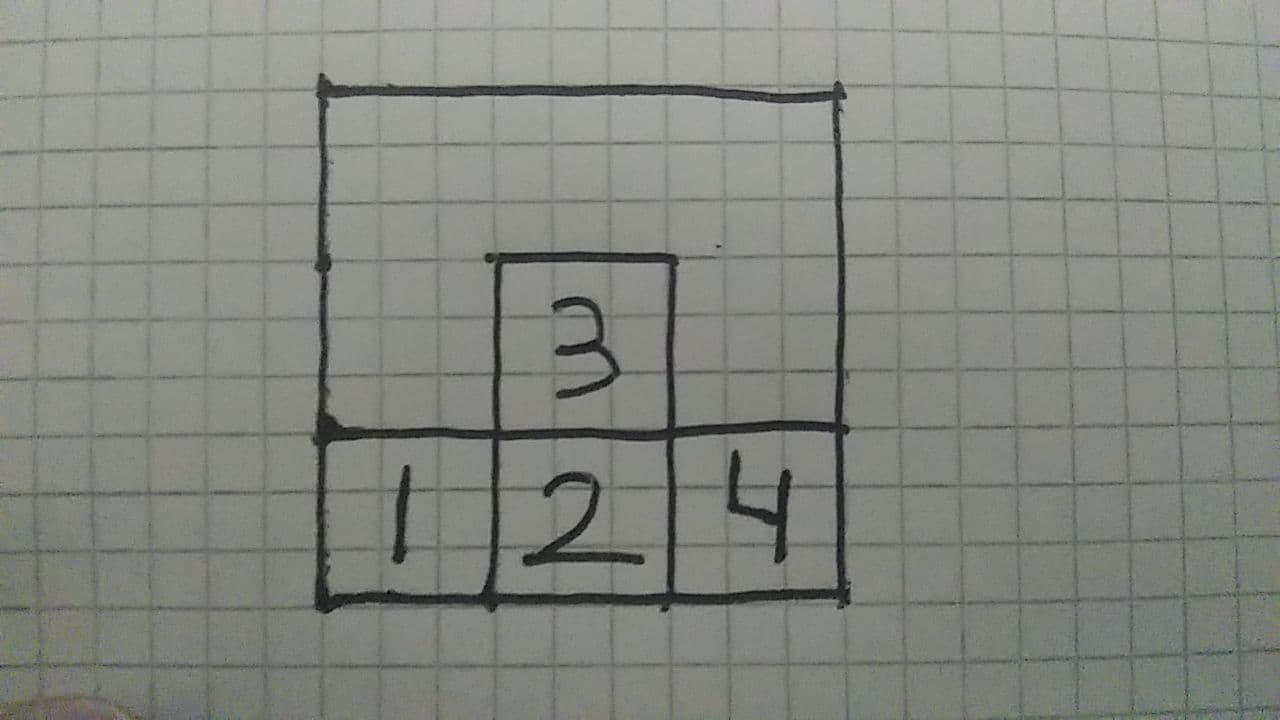
\includegraphics[width=6cm]{../images/sample1/initial.jpg}
		}
		%  No blank line
		\subfloat[Stato finale]{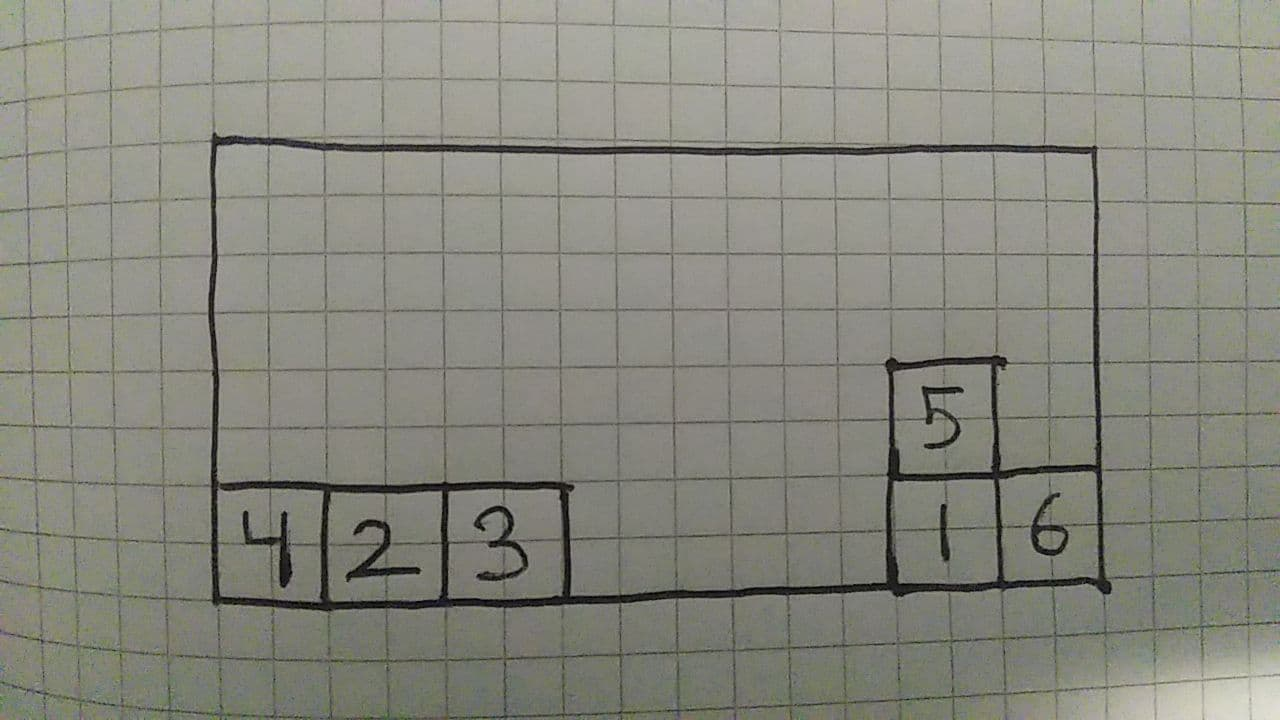
\includegraphics[width=6cm]{../images/sample1/goal.jpg}
		}    
		\protect\caption{Configurazioni per il secondo test}
		\label{fig:exp2}
	\end{figure}
	
	\noindent Le due immagini vengono elaborate e codificate correttamente nei seguenti stati:
	\begin{minted}{python}
	initial = ((1,0,0), (2,0,1), (3,1,1), (4,0,2), 3)
	goal    = ((3,0,0), (4,0,1), (2,1,1), (1,0,2), 3)
	\end{minted}
	Le performance dei vari algoritmi di ricerca sono riassunte nella tabella \ref{tab:exp2}.
	\begin{table}[H]
		\centering
		\def\arraystretch{1.5}
		\begin{tabular}{|c|c|c|c|c|}
			\hline
			\textbf{Algoritmo} & \bm{$n$} & \bm{$m$} & \bm{$\mu$} & \bm{$l$} \\
			\hline
			DFS & 469 & 390 & 208 & 271 \\
			\hline
			BFS &  716 & 411 & 264 & 7 \\
			\hline
			IDS &  27596 & 8 & 6 & 7 \\
			\hline
			UCS &  703 & 408 & 264 & 7 \\
			\hline
			A* &  67 & 120 & 61 & 7 \\
			\hline
			RBFS &  96 & 35 & 18 & 7 \\
			\hline
			
		\end{tabular}
		\caption{Performance algoritmi di ricerca nel secondo test}
		\label{tab:exp2}
	\end{table}
	
	
	\subsubsection{Terzo test}
	Nel terzo test si vuole vedere come si comportano gli algoritmi in una configurazione con 6 blocchi (figura \ref{fig:exp3}). In risultati (tabella \ref{tab:exp3}) della DFS  non sono riportati in quanto non è stata in grado di fornire una soluzione dopo svariati minuti di esecuzione.
	\begin{figure}[H]
		\centering
		\subfloat[Stato iniziale]{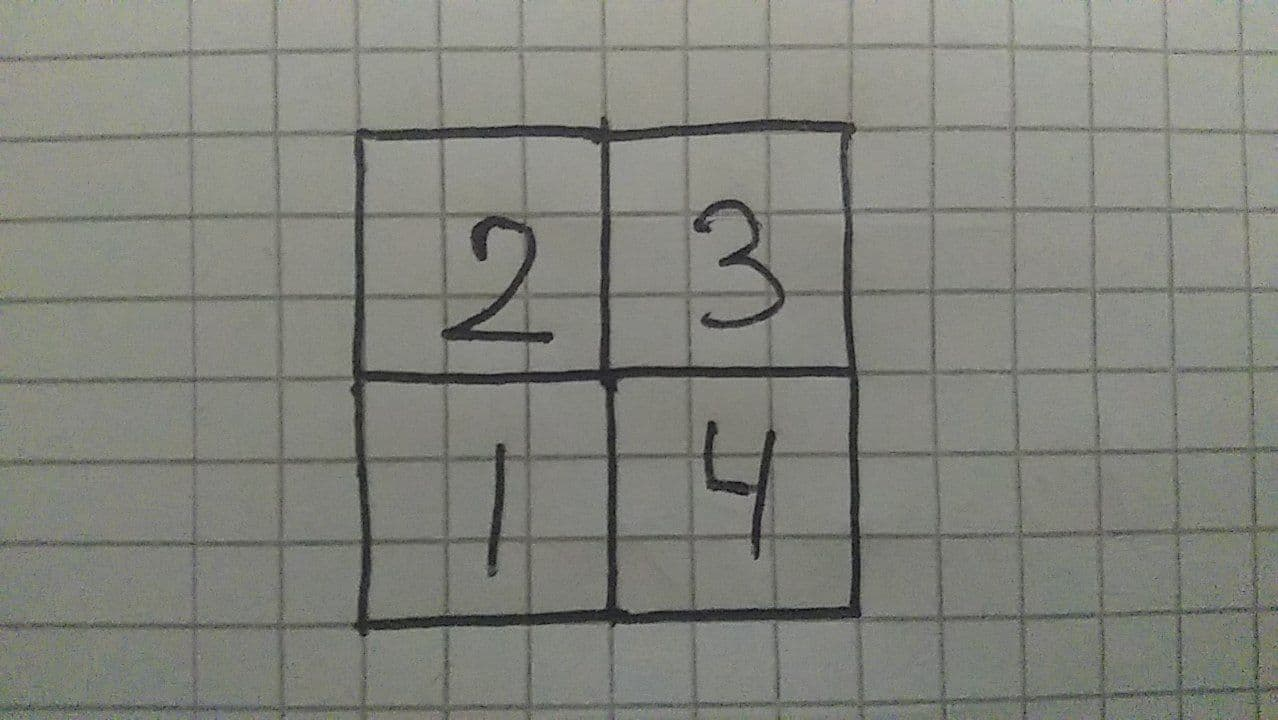
\includegraphics[width=6cm]{../images/sample2/initial.jpg}
		}
		%  No blank line
		\subfloat[Stato finale]{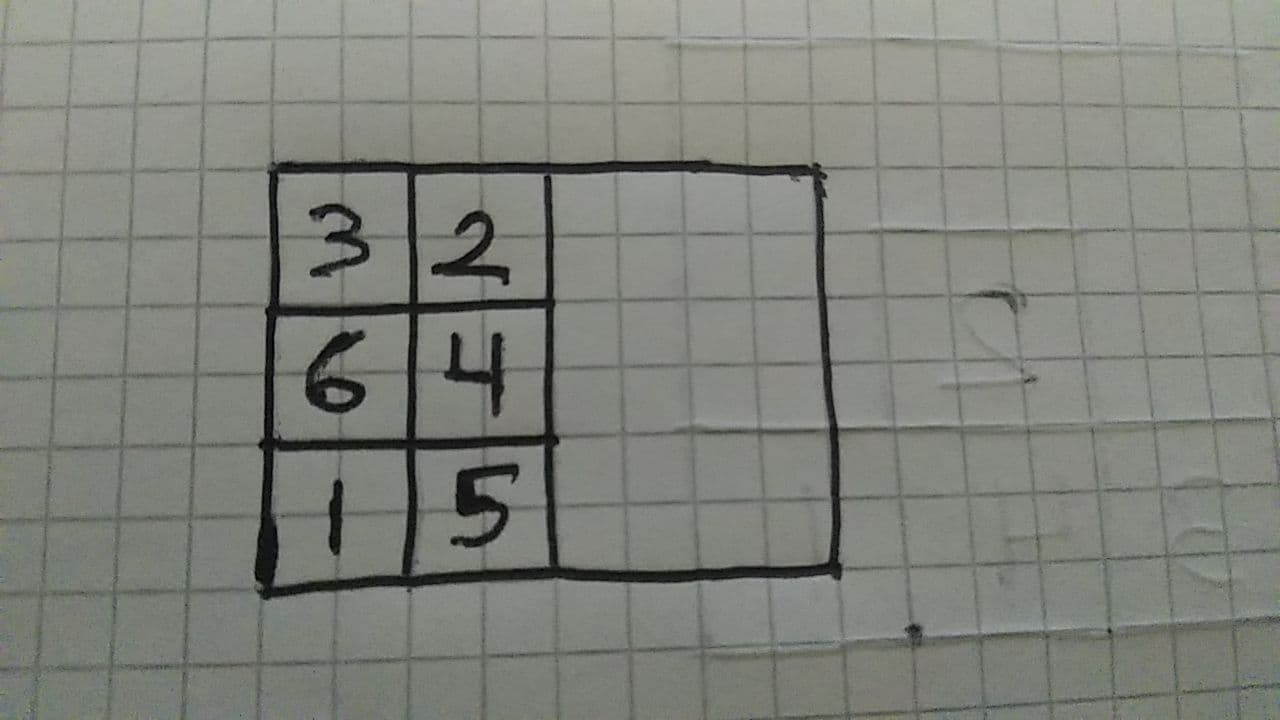
\includegraphics[width=6cm]{../images/sample2/goal.jpg}
		}    
		\protect\caption{Configurazioni per il primo test}
		\label{fig:exp3}
	\end{figure}
	
	\noindent Le due immagini vengono elaborate e codificate correttamente nei seguenti stati:
	\begin{minted}{python}
   initial = ((1,0,0), (6,1,0), (5,0,1), (4,0,2), (2,0,3), (3,1,3), 4)
   goal    = ((1,0,0), (6,1,0), (3,2,0), (5,0,1), (4,1,1), (2,2,1), 4)
	\end{minted}

	\begin{table}[H]
		\centering
		\def\arraystretch{1.5}
		\begin{tabular}{|c|c|c|c|c|}
			\hline
			\textbf{Algoritmo} & \bm{$n$} & \bm{$m$} & \bm{$\mu$} & \bm{$l$} \\
			\hline
			DFS & - & - & - & - \\
			\hline
			BFS & 441 & 1744 & 941 & 3 \\
			\hline
			IDS &  1011 & 4 & 3 & 3 \\
			\hline
			UCS &  454 & 1824 & 1007 & 3 \\
			\hline
			A* &  7 & 32 & 16 & 3 \\
			\hline
			RBFS & 4 & 31 & 16 & 3   \\
			\hline
		\end{tabular}
		\caption{Performance algoritmi di ricerca nel terzo test}
		\label{tab:exp3}
	\end{table}


	\subsubsection{Quarto test}
	Il quarto test (figura \ref{fig:exp4}) è stato condotto in una configurazione con uno stato in meno della precedente, ma la soluzione migliore che richiede qualche azione in più. Anche in questo caso la DFS fallisce nel fornire un risultato in tempi utili. I risultati sono riportati nella tabella \ref{tab:exp4}.
	\begin{figure}[H]
		\centering
		\subfloat[Stato iniziale]{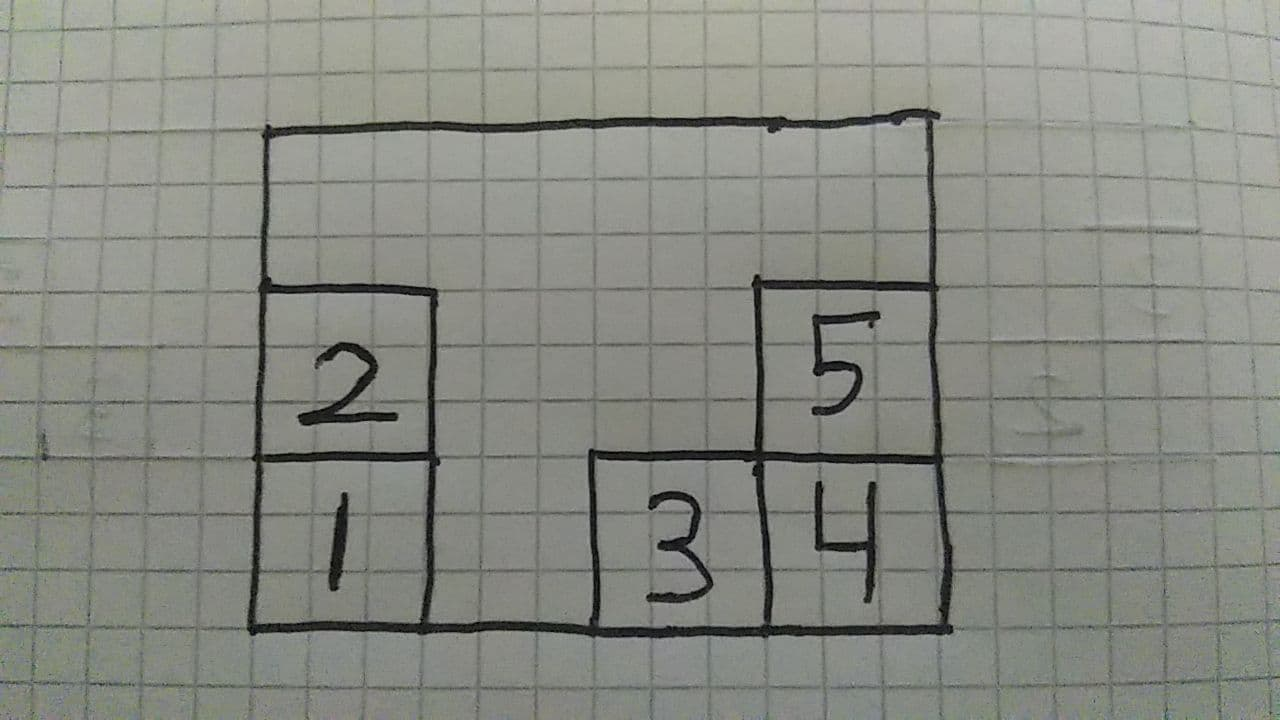
\includegraphics[width=6cm]{../images/sample3/initial.jpg}
		}
		%  No blank line
		\subfloat[Stato finale]{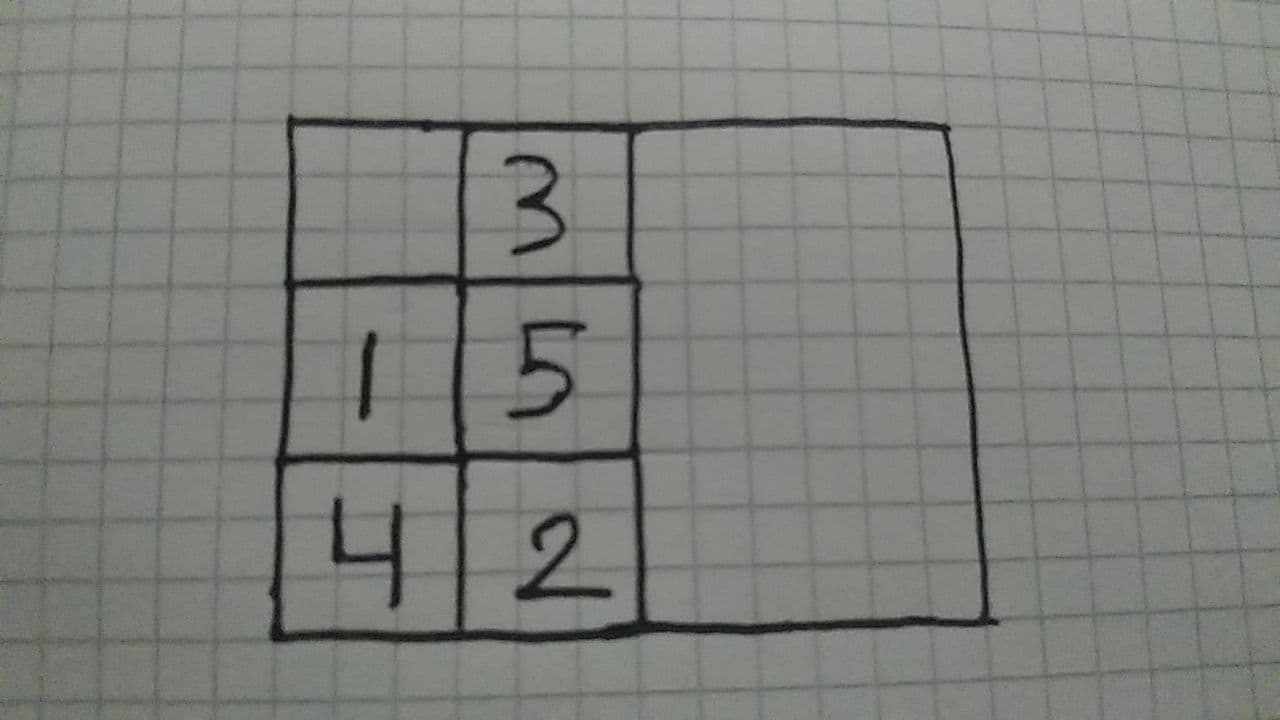
\includegraphics[width=6cm]{../images/sample3/goal.jpg}
		}    
		\protect\caption{Configurazioni per il quarto test}
		\label{fig:exp4}
	\end{figure}
	
	\noindent Le due immagini vengono elaborate e codificate correttamente nei seguenti stati:
	\begin{minted}{python}
   initial = ((1,0,0), (6,1,0), (5,0,1), (4,0,2), (2,0,3), (3,1,3), 4)
   goal    = ((1,0,0), (6,1,0), (3,2,0), (5,0,1), (4,1,1), (2,2,1), 4)
	\end{minted}
	Le performance dei vari algoritmi di ricerca sono riassunte nella tabella:
	\begin{table}[H]
		\centering
		\def\arraystretch{1.5}
		\begin{tabular}{|c|c|c|c|c|}
			\hline
			\textbf{Algoritmo} & \bm{$n$} & \bm{$m$} & \bm{$\mu$} & \bm{$l$} \\
			\hline
			DFS & - & - & - & - \\
			\hline
			BFS & 5514 & 10002 & 5556 & 6 \\
			\hline
			IDS &  80128 & 7 & 5 & 6 \\
			\hline
			UCS &  7555 & 11819 & 6879 & 6 \\
			\hline
			A* &  35 & 163 & 84 & 6 \\
			\hline
			RBFS & 7 & 55 & 30 & 6 \\
			\hline
			
		\end{tabular}
		\caption{Performance algoritmi di ricerca nel quarto test}
		\label{tab:exp4}
	\end{table}


	\subsubsection{Quinto test}
	Infine è stato realizzato un test in una configurazione particolarmente complessa (figura \ref{fig:exp5}), infatti le ricerche non in informate si rivelano inadeguate e non riescono a fornire una situazione in tempi accettabili, pertanto sono state riportate solo le informazioni delle ricerche informate (tabella \ref{tab:exp5}) 
	\begin{figure}[H]
		\centering
		\subfloat[Stato iniziale]{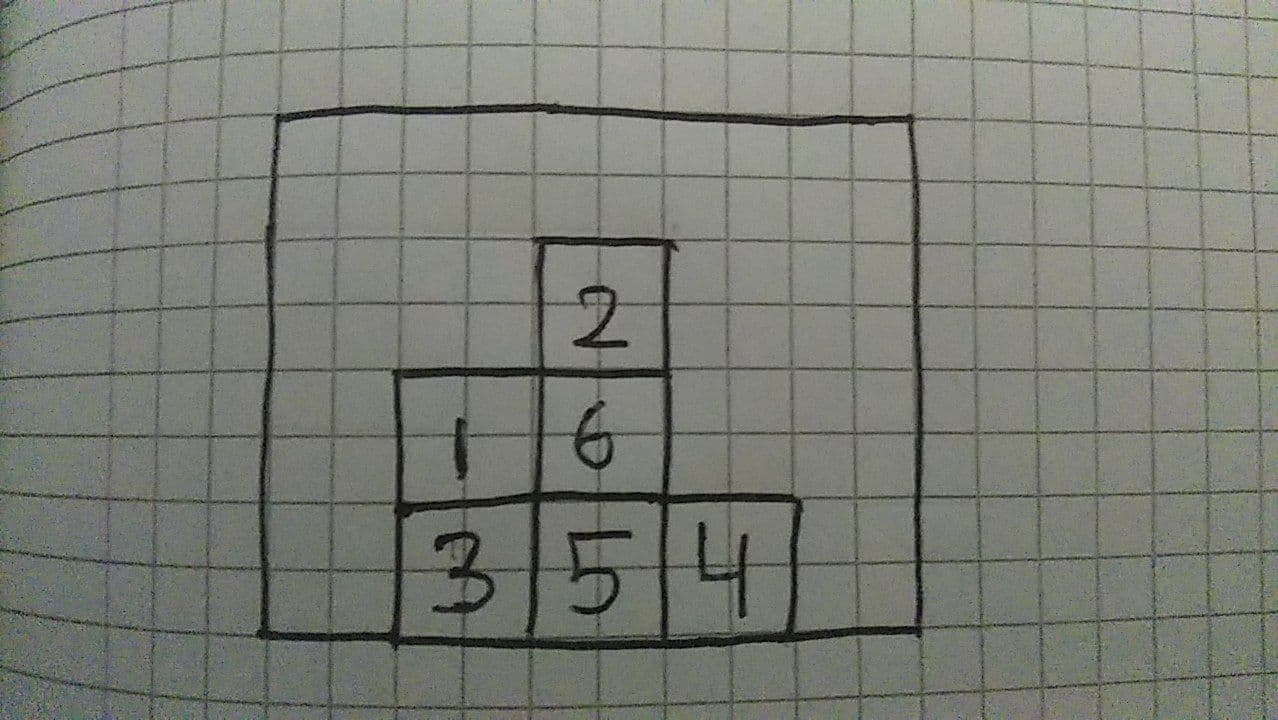
\includegraphics[width=6cm]{../images/sample4/initial.jpg}
		}
		%  No blank line
		\subfloat[Stato finale]{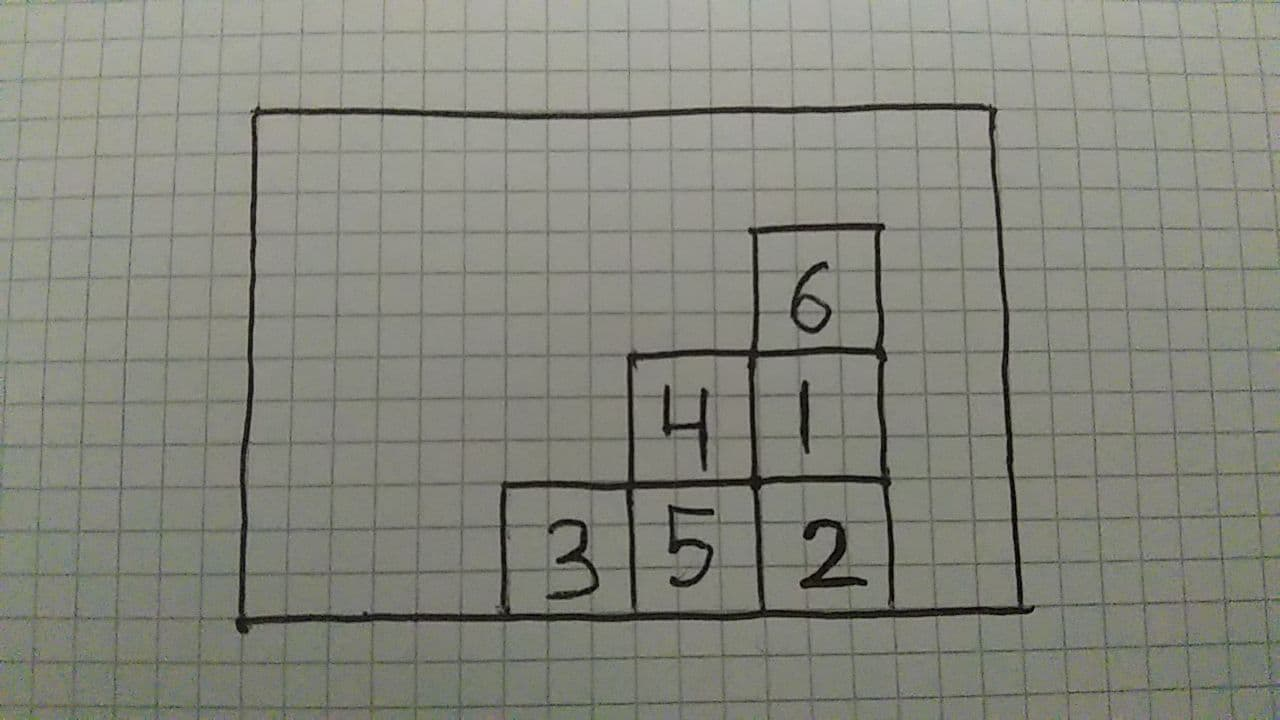
\includegraphics[width=6cm]{../images/sample4/goal.jpg}
		}    
		\protect\caption{Configurazioni per il quinto test}
		\label{fig:exp5}
	\end{figure}
	
	\noindent Le due immagini vengono elaborate e codificate correttamente nei seguenti stati:
	\begin{minted}{python}
initial = ((1,0,1), (6,0,2), (2,1,2), (4,0,3), (5,1,3), (3,0,4), 6)
goal    = ((3,0,2), (5,0,3), (4,1,3), (2,0,4), (1,1,4), (6,2,4), 6)
	\end{minted}
	
	\begin{table}[H]
		\centering
		\def\arraystretch{1.5}
		\begin{tabular}{|c|c|c|c|c|}
			\hline
			\textbf{Algoritmo} & \bm{$n$} & \bm{$m$} & \bm{$\mu$} & \bm{$l$} \\
			\hline
			A* & 3969 & 31281 & 15978 & 9 \\
			\hline
			RBFS &  29200 & 196 & 109 & 9 \\
			\hline
			
		\end{tabular}
		\caption{Performance di A* e RBFS nel quinto test}
		\label{tab:exp5}
	\end{table}

	\subsection{Considerazioni}
	\subsubsection{Considerazioni sugli algoritmi di ricerca}
	Per quanto riguarda gli algoritmi di ricerca si possono effettuare le seguenti considerazioni:
	\begin{itemize}
		\item La DFS, che ha una complessità in tempo più bassa degli altri algoritmi, tende ad avere una dimensione della frontiera (sia massima che media) ed un numero di nodi espansi più bassi rispetto a quella di altri algoritmi come la BFS e la UCS. Di contro la lunghezza delle soluzioni che trova sono esageratamente maggiori di quelle degli altri algoritmi, poiché la DFS non è ottimale neanche rispetto alla lunghezza della soluzione. Tutti gli altri algoritmi invece, quando trovano una soluzione, essa è sempre ottimale (questo anche per come è stata definita la funzione di costo che rende la BFS ottimale).
		\item BFS e UCS tendono ad avere prestazioni simili, in quanto la funzione di costo utilizzata dalla UCS ha costo unitario per ogni azione, quindi essenzialmente equivale ad una BFS, cambia solo il momento nel quale viene fatto il goal test (al momento dell'espansione nell'UCS e al momento della scoperta del nodo nella BFS).
		\item La complessità in spazio della IDS è $O(d)$ infatti dimensione massima e media della frontiera sono sempre più o meno simili alla lunghezza della soluzione. Di contro il numero di nodi espansi è elevatissimo in quanto l'albero di ricerca viene interamente espanso tutte le volte per le profondità che vanno da $0$ a $d-1$.
		\item A* e RBFS tendono a far meglio di tutte le altre ricerche non informate, e la differenza è più marcata più è complessa l'istanza del mondo che si prende in esame.
		\item L'RBFS rispetto all'A* tende ad avere prestazioni migliori per quanto riguarda la memorizzazione (quindi la dimensione della frontiera), ma di contro il numero di nodi espansi è estremamente maggiore.
		\item Un altro fatto interessante da notare è come nel quinto esperimento, sebbene l'A* espanda molti meno nodi della RBFS, quest'ultima impiega molto meno tempo a terminare la sua esecuzione. La stessa cosa avviene per UCS e BFS, che espandono un numero di nodi pressoché identico, ma la UCS spesso richiede qualche secondo di esecuzione in più. La spiegazione più sensata che ho trovato è che probabilmente ciò è causato da un overhead nel mantenere ordinata la coda di priorità in A* e UCS.
	\end{itemize}

	\subsubsection{Considerazioni generali}
	Risulta evidente come in istanze del mondo più complesse, ovvero che richiedono soluzioni più lunghe o dove le possibile azioni ad ogni stato sono maggiori, tutti gli algoritmi falliscono nel trovare soluzioni in tempo fattibile. Quelli che si comportano meglio sono A* e RBFS, che però possono anche richiedere esecuzioni di diversi minuti prima di trovare una soluzione. La ragione di ciò probabilmente risiede sul come è stato modellato il problema, che nelle istanze più complesse fa esplodere la dimensione dello spazio degli stati. Per illustrare il perché con un esempio, si consideri il seguente stato di larghezza 6:
	\begin{minted}{python}
	((1,0,0), (2,0,1), (3,0,2), (4,0,3), (5,0,4), (6,0,5), 6)
	\end{minted}
	tutti blocchi sono disposti sulla superficie del mondo in maniera incrementale da sinistra verso destra. Ogni blocco può essere spostato sopra ognuno degli altri 5 blocchi, quindi le azioni possibili sono $5 \times 6 = 30$. Se si decide di prendere un qualsiasi blocco $x$ e spostarlo sopra un altro blocco $y$, il blocco $y$ non potrà più essere spostato, mentre gli altri 5 blocchi potranno essere spostati, ognuno in 5 possibili posizioni, quindi si hanno $5 \times 5 = 25$ possibili azioni e, tenendo in considerazione il percorso dallo stato di partenza, le sequenze di azioni possibili in totale sono $30 \times 25 = 750$. Si supponga ora di prendere un terzo blocco $z$ e di porlo dove nel primo stato era posizionato $x$, ragionando come prima anche in questo caso si hanno $5 \times 5 = 25$ possibili azioni nello stato, per un totale di $30 \times 25 \times 25 = 18750$ possibili azioni. Si supponga ora di riporre $x$ dove nello stato originale si trovava $z$, si ritorna in una configurazione come quella iniziale ma con $x$ e $z$ invertiti di posizione, quindi si hanno di nuovo $5 \times 6 = 30$ possibili azioni, per un totale di $30 \times 25 \times 25 \times 30 = 562500$.\\Quindi dall'esempio risulta evidente come basta poco per creare uno spazio degli stati intrattabilmente grande. Un possibile modo per rendere più efficiente l'esecuzione del programma potrebbe essere quello di definire una migliore funzione euristica, in quanto, utilizzando il numero di blocchi in posizione errata, il valore massimo della funzione è pari al numero di blocchi presenti nell'istanza del mondo, quando la soluzione con il minor numero di azioni potrebbe essere anche più lunga.
	
	\section{Uso del programma}
	\subsection{Linea di comando}
	Per utilizzare il programma da linea di comando va utilizzato il file \verb*|main.py|, il quale accetta i seguenti argomenti:
	\begin{itemize}
		\item \textbf{-\--initial, -i}\\Permette di specificare il file dell'immagine che rappresenta lo stato iniziale
		\item \textbf{-\--goal, -g}\\Permette di specificare il file dell'immagine che rappresenta lo stato finale
		\item \textbf{-\--a, algorithm}\\Permette di specificare quale algoritmo di ricerca utilizzare. Le possibili opzioni sono le seguenti:
		\begin{itemize}
			\item astar
			\item bfs
			\item dfs
			\item ids
			\item ucs
			\item rbfs
		\end{itemize}
		\item \textbf{-\--degub, -d}\\Permette visualizzare il processo di elaborazione delle immagini
		\item \textbf{-\--output, -o}\\Permette di visualizzare la soluzione tramite una rappresentazione grafica degli stati
		\item \textbf{-\--help, -h}\\Premette di visualizzare una breve guida che illustra il funzionamento degli argomenti del comando
	\end{itemize}
	
	\subsection{GUI}
	Per utilizzare il programma tramite interfaccia grafica va eseguito il file \verb*|launch.py|. A quel punto si avvierà un'interfaccia grafica realizzata tramite il modulo Python Tkinter. Per utilizzare il programma è necessario:
	\begin{enumerate}
		\item Selezionare l'immagine raffigurante lo stato iniziale
		\item Selezionare l'immagine raffigurante lo stato finale
		\item Selezionare tramite il menu a tendina l'algoritmo da utilizzare
		\item Premere il tasto di avvio della ricerca
	\end{enumerate}
	\begin{figure}[H]
		\centering
		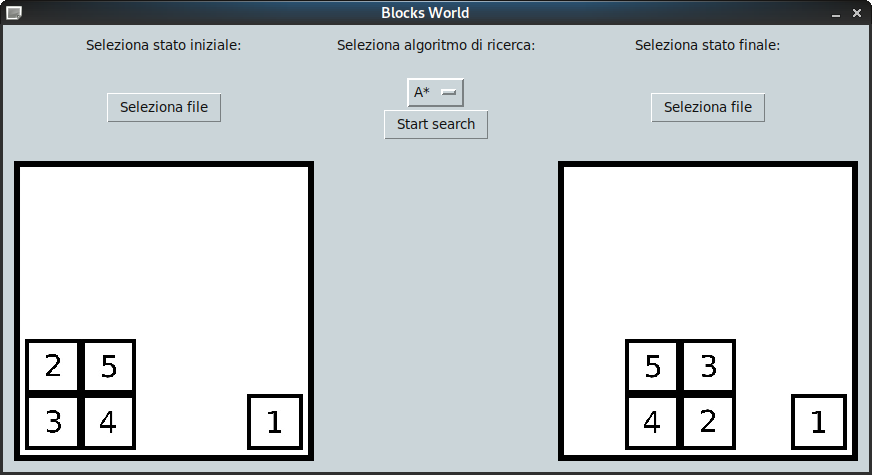
\includegraphics[width=12cm]{./images/gui.png}
		\caption{Interfaccia grafica del programma}
	\end{figure}
	
\end{document}